%\documentclass{article}
%\usepackage{graphicx} % Required for inserting images

%\documentclass[11pt,twoside]{book}

\documentclass[11pt, twoside]{book}
\usepackage[english]{babel}
\usepackage[utf8]{inputenc}
\usepackage[T1]{fontenc}
    
\usepackage[svgnames,hyperref]{xcolor} 
\usepackage{epsfig,graphicx}
%\usepackage[mono=false]{libertine} % new linux font, ignore mono

%\bibliographystyle{ieeetr}

%\usepackage{luatex85}

%\renewcommand{\baselinestretch}{1.05}
\usepackage{amsmath,amsthm,amssymb,mathrsfs,amsfonts}
\usepackage{tabularx}
\usepackage{tikz}
\usepackage{pgfplots}
\pgfplotsset{compat=1.18}
\usepackage{multicol} % two-col ToC
\usepackage{bm}
\usepackage{imakeidx} % before hyperref
\usepackage{hyperref}
% link colors settings
\hypersetup{
    colorlinks=true,
    citecolor=magenta,
    linkcolor=blue,
    filecolor=green,
    urlcolor=cyan,
    % hypertexnames=false,
}
%\usepackage[capitalise]{cleveref}
%\usepackage{subcaption}
%\usepackage{enumitem}
\usepackage{mathtools}
\usepackage{subfiles}

% adjust margin
\usepackage[margin=2.3cm]{geometry}
\headheight13.6pt

% figures inside text
\usepackage{wrapfig}
\usepackage{listings}
\usepackage{xcolor}

% --- Definizione dei colori (opzionale ma consigliata) ---
\definecolor{codegreen}{rgb}{0,0.6,0}
\definecolor{codegray}{rgb}{0.5,0.5,0.5}
\definecolor{codepurple}{rgb}{0.58,0,0.82}
\definecolor{backcolour}{rgb}{0.95,0.95,0.92}

% --- Stile del codice ---
\lstdefinestyle{mystyle}{
	backgroundcolor=\color{backcolour},   % Colore di sfondo (toglilo se vuoi sfondo bianco)
	commentstyle=\color{codegreen},       % Colore commenti
	otherkeywords={std::vector},
	keywordstyle=\color{blue},         % Colore keyword (int, float, class...)
	numberstyle=\tiny\color{codegray},    % Stile numeri di riga
	stringstyle=\color{codepurple},       % Colore stringhe
	basicstyle=\ttfamily\footnotesize,    % Font monospaziato e dimensione
	breakatwhitespace=false,         
	breaklines=true,                      % Manda a capo le righe troppo lunghe
	captionpos=b,                         % Posizione della caption (bottom)
	keepspaces=true,                 
	numbers=left,                         % Numeri di riga a sinistra
	numbersep=5pt,                  
	showspaces=false,                
	showstringspaces=false,
	showtabs=false,                  
	tabsize=4                             % Dimensione tabulazione
}

% Attiva lo stile appena definito
\lstset{style=mystyle}

\newcommand{\CC}{\mathcal{C}}


\title{Exercises NMSM 2025-2026}
\author{Lorenzo Rizzi - 2156773}
\date{December 2025}

\begin{document}


\setcounter{chapter}{1}
\date{\today}


\maketitle
\tableofcontents
%%%%%%%%%%%%%%%%%%%%%%%%%%%%
%\frontmatter


%\mainmatter
\chapter{Off-lattice Monte Carlo simulations}


\section{The Hard Sphere model}

The \textit{Hard Sphere model} is a paradigmatic model in Soft Matter (despite the naming would not suggest so). The interaction energy between two hard spheres is zero if the separation distance is larger than the diameter of the particle $\sigma$ and infinite otherwise. Set $\sigma=1$ as the unit of length. Using the Hard Sphere model, one can simplify the Metropolis acceptance rule as follows:
\begin{itemize}
	\item reject every displacement that brings any two particles closer than $\sigma$; call it an overlap. You can assign a very large energy to the configuration if an overlap is present, thus overlap can be spotted more easily.
	\item accept every displacement that keeps every pair of particles at a distance larger than $\sigma$ or that removes an overlap.
\end{itemize}
An acceptable state for a Hard Sphere system has zero energy and is homogeneously distributed in the simulation box. Consider a system of $N = 200$ Hard Spheres in three dimensions. Starting from random conformations, simulate the system at different number density $\rho = \frac{N}{V}: (i)\> \rho = 0.05\sigma^{-3} (ii)\> \rho = 0.4\sigma^{-3}$ and $(iii)\> \rho = 0.62\sigma^{-3}$. Use a simple cubic box and pay attention to set a suitable maximum displacement. Check that
the energy reaches zero (equilibration) before collecting data. Compute the radial distribution function
$g_2(r)$, discussed in class and describe what changes between the three different states.
\textbf{\\ Resolution \\}
The model we are implementing is based on the hard-sphere nature of the constituent molecules. Formally, we can write the Hamiltonian of the system as:
$$
\mathcal{H} = T + V = \sum_i \frac{1}{2}mv_i^2 + U
$$
where $T$ represents the standard kinetic energy and $U$ is the total potential energy of the system, composed of pair-wise interactions $U = \sum_{i\neq j}U_{ij}$. Specifically, the hard-sphere condition is realized by imposing\footnote{Note that we have rescaled the spatial lengths by choosing $\sigma = 1$, where $\sigma$ is the molecular diameter. In this report, all lengths will therefore be dimensionless}:
\begin{equation}
	U_{ij}=
	\begin{cases}
		\infty \>\> \text{       if       } \>\> |\vec r_i - \vec r_j | < 1 \\
		0 \>\> \text{        if       } \>\>|\vec r_i - \vec r_j | > 1 
	\end{cases}
\end{equation}
Thus, the molecules interact only to avoid spatial overlaps but are otherwise free to move without experiencing any force. In the NVT ensemble (the one sampled with Metropolis), the probability distribution function in phase space $(\vec r_i, \vec p_i)$ is given by the Boltzmann formula:
$$
p(\{\vec{r},\vec{p}\}) = \frac{1}{Z}\exp(-\beta \mathcal{H}(\{\vec r, \vec p\}))
$$ 
However, in this specific context, we are interested only in the marginalized configurational probability distribution, i.e., the probability of observing a specific configuration in coordinate space:
$$
p(\{\vec{r}\}) = \int d\vec{p}_1d\vec{p}_2 \dots d\vec p_n \> p(\{\vec{r},\vec{p}\}) 
$$
This expression factorizes conveniently due to the fact that the potential energy depends only on the configuration $\{\vec r_i\}$ and the kinetic energy only on the momenta $\{\vec p_i\}$:
$$
p(\{\vec{r}\}) = p(\vec{r}_1, \vec{r}_2, \dots \vec{r}_n) = \frac{1}{Z_{conf}}\exp(-\beta U) = \frac{1}{Z_{conf}}\exp\left(-\beta \sum_{i\neq j}U_{ij}\right)
$$
This is the probability distribution we want to sample from. In the hard-sphere model, this further simplifies to:
\begin{equation}
	p(\{\vec{r}\}) =
	\begin{cases}
		const \neq 0  \>\>\> \text{ if no overlap occurs} \\
		0  \>\>\> \text{ if even one overlap occurs} \\
	\end{cases}
	\label{eq1}
\end{equation}
This implies that all \textit{acceptable} states (i.e. configurations with no overlaps) are equiprobable. The Metropolis algorithm that will be implemented in the next section is designed to generate samples drawn precisely from this probability distribution. Before proceeding with the implementation of the algorithm, a few remarks:
\begin{itemize}
	\item The derivation of the marginalized configurational probability was carried out in the canonical ensemble (NVT). However, due to the specific form of the potential, there is effectively no distinction in this context between the microcanonical (NVE) and the canonical ensembles. Indeed, the dependence on the thermal parameter $\beta$ vanishes because the potential is either zero or infinite, rendering the Boltzmann factor independent of temperature for all allowed configurations.
	\item We construct Markov chains designed to sample from the PDF in Eq.\ref{eq1}. It is important to note that this type of MC simulation is inherently static, meaning that we are sampling only the configurational component of the full distribution. Consequently, our MCMC algorithm yields configurations sampled with the correct probability, but no information regarding velocities can be inferred from these purely spatial samples. We can, therefore, compute only static or structural properties (such as the radial distribution function) that depend solely on the configurational subspace.
\end{itemize}

\subsection{The algorithm}
This section briefly summarizes the implementation of the algorithm in C++. A base structure \texttt{Particle} was defined to store a $d$-dimensional tuple of coordinates. The core class of the codebase is structured as follows:

\begin{lstlisting}[language=C++]
	template<int Dim>
	class NDMolDyn {
		std::vector<Particle> particles;
		std::vector<std::vector<int>> verletLists;
		std::vector<int> headOfChain;
		std::vector<Particle> backupPositions;
	};
\end{lstlisting}
where:\begin{itemize}
	\item The vector \texttt{particles} contains all $N$ constituent particles, where $N$ is defined by the input parameters.
	\item The matrix \texttt{verletLists} implements the \textit{Verlet list strategy}. Specifically, the element \texttt{verletLists[i]} is a list containing the indices of particles that are sufficiently close to the $i$-th particle. Constructing these lists is an effective method to accelerate the force calculation. In fact, when checking if a particle $i$ overlaps with any other particles, we only need to iterate through its Verlet list, whose size is typically much smaller than $N$. This eliminates the need to check all possible particle pairs.
	\item The process of generating the Verlet lists itself can be computationally intensive, potentially introducing a new $O(N^2)$ bottleneck. For this reason, the vector \texttt{headOfChain} implements the \textit{cell list strategy}, which converts the costly Verlet list construction from an $O(N^2)$ operation to a highly efficient $O(N)$ algorithm. The vector \texttt{backupPositions} is used to evaluate whether it is necessary to rebuild the Verlet lists (rebuilding is avoided at each iteration thanks to the presence of a safety parameter, \texttt{skin}). The linked-list structure needed for the cell list approach is not contained in a separate vector $L$, but is included directly into the \texttt{Particle} structure for implementation simplicity:
	\begin{lstlisting}[language=C++]
	template<int Dim>
	struct Particle{
		std::array<double, Dim> position;
		int next = -1;    // -1 means nullptr
	};
	\end{lstlisting}
\end{itemize}
The MC algorithm goes as follows\footnote{This is just a minimal example, the full code is longer because there are additional feature (acceptance rate counter, ...)}:
\begin{lstlisting}[language=C++]
#define vecd std::array<double, Dim>

//Run a single step of MC (thus N proposals)
template<int Dim>
void NDMolDyn<Dim>::singleMCStep(){
	// First of all, select a random particle
	int particle_idx = rand() % m_particles.size();
	vecd old_pos = m_particles[particle_idx].position;
	vecd new_pos;
	for(int k = 0; k < Dim; ++k){
		double delta = (static_cast<double>(rand()) / RAND_MAX) * 2.0 * max_displacement - max_displacement;
		new_pos[k] = old_pos[k] + delta;
		if(new_pos[k] >= m_L){ //PBC
			new_pos[k] -= m_L;
		} else if(new_pos[k] < 0.0){
			new_pos[k] += m_L;
		}
	}
	// Now that we have the new_pos, verify whether there is an overlap
	for(auto it = m_verletLists[particle_idx].begin(); it != m_verletLists[particle_idx].end(); ++it){
		vecd pos_j = m_particles[*it].position;
		double d2 = dist_sq_pbc(new_pos, pos_j);
		if(d2 < 1.0){ //Overlap detected! Return and don't do anything
			return;
		}
	}
	// If we reach this point, we can accept the move
	m_particles[particle_idx].position = new_pos;
	// Finally, check whether we need to rebuild the verlet lists
	double trigger = distance_square_pbc(m_backupParticles[particle_idx], new_pos);
	if (trigger > m_skin/2 * m_skin/2) {
		// Rebuild the verlet lists
		buildVerletLists();
	}
}
\end{lstlisting}

The simulation can be run in an arbitrary number of dimension, but we'll use $d = 2$ or $d=3$ for the sake of simplicity. The parameters that we can modify can be summarized:


\begin{table}[h]
	\centering
	\begin{tabular}{ll}
		$\rho$ & Density \\
		$N$    & Number of particles   \\
		$r_{cut}$ & Cut-off radius, Verlet's technique    \\
		$r_{skin}$ & Skin, Verlet's technique \\
		$M$ & Number of cell per dimension \\
		$MCSteps$ & Number of MC steps to perform (1 MCStep = $N$ proposals)      
	\end{tabular}
\end{table}


When the function \texttt{buildVerletLists()} is called, the program will start filling the object \texttt{std::vector<std::vector<int>> verletLists}. In particular, the list \texttt{verletLists[i]} will consist of all particles whose position $r_j$ is such that:
$$
|\vec r_j - \vec r_i| < r_{cut} + r_{skin}
$$
The parameter $r_{cut}$ should be chosen as to represent a characteristic length over which the interaction dies out. In this specific case, since the pair-wise hard-sphere interaction is non zero only when $|\delta r| < 1$ (diameter of the molecules), we can safely set $r_{cut}=1$. The skin parameter is a performance parameter, meaning that it sets how frequently one has to update the Verlet lists (the less, the better). In this code, I've used to rule according to which when the total displacement of a molecules (with respect to the position occupied the last time \texttt{buildVerletList()} was called) is larger than half of the skin parameter, then the Verlet lists must be rebuilt from scratch. A good choice is $r_{skin} = 0.5$ (but this depends on the specific run). In order for the algorithm to work, a few sanity check are in order:
\begin{itemize}
	\item The Verlet lists are built upon the cell lists, meaning that the neighbours of a particle are selected by only checking adjacent cells. If the linear size of the cells is too small, then we might be losing essential interactions. Specifically, we require:
	\begin{equation}
		M < \Bigl\lfloor \frac{L}{r_{cut} + r_{skin}} \Bigr\rfloor
	\end{equation}
	\item At each MC step, $N$ particles are randomly selected and a spatial move is proposed according to a parameter \texttt{max\_displacement}. In order for this move not to break the Verlet list inner working, we request:
	\begin{equation}
		\text{max\_displacement} < \frac{1}{2} d_{skin}
	\end{equation}
\end{itemize}
The program will automatically perform those sanity check at the beginning of the simulation and signal to the user whether a violation has been detected. 

\subsection{Qualitative analyis}
We set $N = 200$ particles and investigate the behavior of the system in $3D$ across three different number densities: $\rho = 0.62, \rho = 0.4$, and $\rho = 0.05$. The simulation executes the MCMC algorithm and records the coordinates of all particles at specified intervals, dumping them into a \texttt{traj.xyz} file. This output is particularly useful when analyzed with \texttt{OVITO}, a free software package capable of reading \texttt{.xyz} trajectory files and rendering the simulation in $3D$.\footnote{The native $2D$ rendering option was implemented using the SFML library. Instead, due to the complexity of real-time $3D$ rendering, I relied on an external third-party software.} The resulting configurations for the three defined densities are visualized in Fig.\ref{fig:OVITO}: the results qualitatively confirm that higher concentration leads to denser molecular packing. Table.\ref{table:table1} presents the parameters defining the MC chain along with key diagnostic quantities. These diagnostics include the acceptance rate and the rebuild probability (which quantifies the frequency of the computationally expensive Verlet list updates).
\begin{table}
	\centering
	\begin{tabular}{|c|c|c|c|c|c|}
		\hline
		$\rho$ &  Max Displacement & Skin & M & Rebuilding & Acceptance rate\\
		\hline
		$0.05$ &  0.4 & 1 & 5 &14 \%&$0.92 \pm 0.02$ \\

		$0.4$  &  0.35 & 0.8 & 4 & 10 \%&$0.48 \pm 0.05$ \\
		
		$0.62$  &  0.2 & 0.5 & 4&4\%&$0.38 \pm 0.06$ \\ 
		\hline
	\end{tabular}
	\caption{\textit{A list of the parameters governing the Verlet and cell list techniques that were implemented to enhance code performance ($\texttt{max\_displacement, skin, M}$). The total number of MC steps and $r_{cut}$ were held constant at $10^5$ and $1$, respectively. In addition, two diagnostic parameters were monitored to ensure the Markov chain explored the space correctly and that the acceleration technique was effective: the acceptance rate and the rebuilding factor. The acceptance rates for the higher densities ($\rho = 0.4$ and $\rho = 0.62$) can be considered satisfactory, whereas the rate observed for $\rho = 0.05$ is rather high. While in ordinary MC simulations this might suggest the algorithm is exploring the space too slowly, this is not the case here: the low number density implies extremely rare interactions, hence a higher acceptance rate.}}
	\label{table:table1}
\end{table}
\begin{figure}
	\centering
	\includegraphics[scale=0.33]{./FIG/gas.png}
	\includegraphics[scale=0.33]{./FIG/liquid.png}
	\includegraphics[scale=0.33]{./FIG/solid.png}
	\caption{\textit{3D rendering (under periodic boundary condition) performed by OVITO starting from three MC chains. From the left to the right, $\rho = 0.05, \rho = 0.4, \rho = 0.62$ and $N$ is kept constant at $N=200$. The spatial lengths are all rescaled in such a way that $\sigma=1$, where $\sigma$ is the molecules diameter.}}
	\label{fig:OVITO}
\end{figure} 
With the obtained MC chains for the spatial configurations, we can analyze the structural properties of the system, starting with the \textit{radial distribution function} $g(r)$. For this purpose, \texttt{OVITO} was used to calculate the instantaneous, frame-by-frame radial distributions. These instantaneous distributions were subsequently averaged (the Python notebook) to yield a smoother, statistically reliable curve. The resulting time-averaged $g(r)$ curves are shown in the right panel of Fig.\ref{fig:g(r)}. For all simulated densities, $g(r)$ vanishes when $r < 1$. This confirms the expected behavior and serves as a successful sanity check for the algorithm. As spatial overlap is strictly prohibited, no pair of particles can stay closer than the molecular diameter ($r_{\star} = 1$), and $g(r)$ is precisely zero within this exclusion zone. 

The behaviour for $r > 1$ suggests the formation of at least two phases (a gaseous phase and a condensed one). When $\rho = 0.05$, $g(r)$ remains close to the asymptotic line $g(r)=1$, which is characteristic of an ideal gas. In other words, at sufficiently low densities, the local density is relatively homogeneous and comparable to the global density $\rho = N/V$. A slight enhancement is observed at $r \approx 1$, which decays back to $1$ as $r\to \infty$; this indicates that the local density in the immediate vicinity of a molecule is slightly higher than the typical (uncorrelated) density of an ideal gas. This effect is a direct consequence of the excluded volume interaction. Consider a particle fixed at $r=0$: in an ideal gas system, a second particle can arbitrarily occupy any point $\vec r$ in space independent of the existence of the first particle at $\vec r = 0$. Consequently, there would be a finite probability $p(V_\sigma)$ of finding the second particle within the region $V_\sigma$, defined as a sphere of radius $\sigma$ centered at the origin. Getting back to a system with excluded volume interactions, this probability $p(V_\sigma)$ must necessarily be zero, since the potential energy of an overlapping configuration is infinite. Consequently, this probability mass $p(V_\sigma)$ is effectively ''redistributed'' into the accessible region of space immediately surrounding the sphere $V_\sigma$.

When $\rho = 0.4$ or $\rho = 0.62$, the radial distribution curves exhibit more complex features. The peak around $r=1$ becomes significantly more pronounced, increasing in height as $\rho$ increases. Furthermore, the curve displays the characteristic behavior of oscillations exponentially damped that asymptotically decay to the value $1$ as $r \to \infty$. This pattern provides us with crucial information regarding the geometric structure of the system. The alternating peaks and valleys correspond to successive \textit{coordination shells}. The first peak represents the nearest neighbors forming a "cage" around the reference particle, while the subsequent peaks represent layers of secondary neighbors. The first valley implies a region of particle depletion: this is expected, as the presence of a tightly packed first shell prohibits other particles from occupying the same volume due to local exclusion. The damping of these oscillations indicates that the positional correlation is eventually lost at long distances.

Clearly enough, the larger the density $\rho$, the more pronounced those oscillations are (since the geometric packing become more and more regular).

\begin{figure}
	\centering
	\includegraphics[width=0.49\linewidth]{./FIG/RDF_plot.pdf}
	\includegraphics[width=0.49\linewidth]{./FIG/RDF_plot_well.pdf}
	\caption{\textit{(Left panel) Radial distribution function for the hard-sphere model as a function of (rescaled) distance $r$ at different values of $\rho$ (but $N = 200$). In all cases, $g(r)=0$ when $r < 1$, thanks to the excluded volume, and the correlation dies out when $r$ gets larger  (Right panel) Radial distribution function for the Van der Waals model (isotropic patchy hard sphere where $\theta_{max} = \frac{\pi}{2}$). Now a clear correlation appears for all three densities in the region $ 1 < r < 1.2$.}}
	\label{fig:g(r)}
\end{figure}
\section{The Patchy Hard Sphere model}
\subsection{Implementation}
To implement the patchy interaction described by the Kern-Frenkel potential, the \texttt{Particle} structure was extended to include a \texttt{Patch} object, which essentially represents a three-dimensional unit vector. Although each particle is decorated with two patches, their diametrically opposite arrangement allows for a significant simplification: for practical purposes, tracking a single unit vector is sufficient to define the orientation. To evaluate the pairwise interaction energy, the function \texttt{getEnergy()} was developed:
\begin{lstlisting}[language=C++]
double NDMolDyn<3>::getEnergy(vecd particle_pos, Patch particle_patch, int particle_idx) const {
	double energy = 0.0;
	for(auto it = m_verletLists[particle_idx].begin(); it != m_verletLists[particle_idx].end(); ++it){
		vecd pos_j = m_particles[*it].position;
		double d2 = dist_sq_pbc(particle_pos, pos_j);
		// If within interaction range (we've already checked for overlaps)
		if (d2 < (1.0 + 0.2)*(1.0 + 0.2)) {
			double cos_angle_1 = computeAngle(particle_patch, particle_pos, pos_j, d2);
			double cos_angle_2 = computeAngle(m_particles[*it].getPatch(), pos_j, particle_pos, d2);
			if (std::abs(cos_angle_1) > m_cosThetaMax && std::abs(cos_angle_2) >  m_cosThetaMax) { 
				energy += -1.0; //Dimensionless energy, assume epsilon_SW = 1
			}
		}   
	}
	return energy;
}
\end{lstlisting}
\subsection{Extreme cases}
Before considering a reasonable set of values for $\theta_{max}$, let's explore the extreme cases, where $\theta_{max} = 0$ and $\theta_{max} = \frac{\pi}{2}$. In the first case, the molecules needs to be completely and perfectly aligned to interact; this is impossible (because of machine precision), so when $\theta_{max} = 0$ we fallback to the previous case where no interactions (apart from the repulsive volume) occurs. However, when $\theta_{max} = \frac{\pi}{2}$ then particles will always interact as long as their distance is smaller than $1+\delta = 1+0.2$ (but larger than 1). This is the case where no patchy-like interactions occur and only a spherically symmetric potential well around the molecules is considered (a sort of Van der Walls gas!)

We fix $\theta_{max} = \frac{\pi}{2}$ and evaluate the radial distribution function at $k_B T = 0.8$ for three different densities\footnote{Energy is rendered dimensionless by normalizing to the potential well depth, that is by setting $\epsilon_{SW} = -1$.}. The results are presented in the right panel of Fig.\ref{fig:g(r)}. Once again, for $r < 1$, the radial distribution vanishes due to the excluded volume interaction. However, particles are now subject to a short-range attractive potential well (energy gain of $-1$) which favors configurations where particles are directly surrounded by other particles. Indeed, Fig.\ref{fig:g(r)} confirms the presence of a region $1 < r < 1.2$ where the local density significantly exceeds the bulk density, suggesting the formation of small molecular clusters. Beyond the interaction range ($r > 1.2$), we recover the typical oscillatory behavior for high densities or the flat asymptotic profile for low densities. 

In Fig.\ref{fig:OVITOisotropic}, we present three simulation snapshots rendered with OVITO, corresponding to the configurations analyzed in the right panel of Fig.\ref{fig:g(r)}, where an isotropic potential well is included. Particles separated by a distance less than $1.2$ are visually connected by a bond, representing a direct (negative) contribution to the potential energy. The case of $\rho = 0.05$ is particularly interesting: although the system remains in a gaseous phase, the presence of a short-range attractive potential renders small molecular clusters thermodynamically stable (and energetically favorable). Consequently, we observe the formation of pairs (dimers), and with rapidly decreasing probability, triplets (trimers) or higher-order structures.

One might argue that the formation of these structures is merely coincidental, potentially occurring even in the absence of a potential well (these apparent bonds could simply result from random spatial fluctuations where particles momentarily approach each other at a distance smaller than $1.2$)\footnote{Bonds in the case where no potential well exists doesn't make much sense, since they do not contribute to the energy of the system. The point I'm trying to prove here is that, when the potential is switched on, the fact that a certain amount of molecules tend to cluster together in small structure cannot be simply explained by pure luck, i.e. particles that eventually come closer.}. To verify that the emergence of these structures is effectively driven by the short-range interaction, we quantify the number of bonds in both cases (i.e., $\epsilon = 0$ and $\epsilon = -1$), defining a bond between two particles whenever their mutual distance is less than $1.2$.

I've run a simulation with $10k$ MC steps under those conditions and averaged the number of bonds $b$ for the last $1000$ steps. When $\epsilon = 0$, we measure $b = 16 \pm 4$, whereas when $\epsilon = -1$ we obtain $b = 52 \pm 5$. This is enough evidence to prove that the short range potential is responsible for the formation of those very small structures (only a few particles wide).

\begin{figure}
	\centering
	\hspace{-0.5cm}
	\includegraphics[scale=0.33]{./FIG/gas_well1.png}
	\hspace{0.1cm}
	\includegraphics[scale=0.33]{./FIG/liquid_well1.png}
	\hspace{0.1cm}
	\includegraphics[scale=0.33]{./FIG/solid_well1.png}
	\hspace{-0.5cm}
	\caption{\textit{3D rendering (under periodic boundary condition) performed by OVITO starting from three MC chains (isotropic potential well + excluded volume). From the left to the right, $\rho = 0.05, \rho = 0.4, \rho = 0.62$ and $N$ is kept constant at $N=200$. The blue bonds connect pair of molecule whose distance is less than $1.2$ (thus interacting particles).}}
	\label{fig:OVITOisotropic}
\end{figure} 

\paragraph{Energy and condensation}
An alternative approach to investigating bonds formation involves the analysis of the system's potential energy. Indeed, a direct relationship exists such that $U = -Nb$, where $b$ denotes the number of bonds. The evolution of the potential energy as a function of MC steps is illustrated in Fig.\ref{fig:3traceplots}, alongside a histogram of the same observable at a temperature of $k_B T = 0.8$. As expected, the MCMC algorithm begins sampling configurations from the correct equilibrium distribution only after a transient period, which depends on the chosen initial state. Following this initial \textbf{burn-in} phase, the trace plots clearly demonstrate that the Monte Carlo chains have converged to the limiting distribution and are sampling effectively. The distribution of the samples is approximately Gaussian, a result consistent with standard expectations in statistical mechanics that serves as a validity check. To obtain a Monte Carlo estimate of the thermal average $\langle U \rangle$, we discard the initial samples (burn-in) and compute the mean over the remaining trajectory. Next, we can compute the average energy $\langle U \rangle$ for different values of $\rho$ and $T$ (Fig.\ref{fig:transphase}). 

\begin{figure}
	\centering
	\includegraphics[scale = .8]{./FIG/Energy_analysis_well.pdf}
	\caption{\textit{Trace plots (on the left) and relative histograms (on the right) for three MC chains sampling from the isotropic potential well system ($\cos(\theta_{max}) = \pi /2$) at fixed temperature $k_B T = 0.8$ for three different values of density $\rho$. Number of particles $N = 200$ and $10000$ MC steps. Both the trace plots and the histograms display the usual behaviour expected from a Markov chain-based algorithm (an initial transient + a thermalized phase).}}
	\label{fig:3traceplots}
\end{figure}

At sufficiently high temperatures (specifically, where ``high'' means much larger than the depth of the potential well), the effect of the short-range potential becomes essentially negligible, as particles have sufficient thermal energy to freely enter and exit the potential well. Consequently, these high-temperature systems effectively behave as systems governed purely by excluded volume interactions. The energy curve should thus relax to an asymptotic value $U_{free}$ that can be interpreted as the energy that the system would have if the probability distribution function on the configuration space was the one associated to the same system with no potential well. When the density is low enough ($\rho = 0.05$), then particles are usually far away from each other and we expect: 
$$
U_{free} = \lim_{T\to\infty} U_{well}(T) = 0
$$
However, when the density grows, the asymptotic energy $U_{free}$ becomes increasingly negative. This is simply due to the fact that, when the system is high-density, there will be a moderate probability that a pair of particles gets closer than $1.2$, thus creating a bond and adding a quanta $\epsilon=-1$ to the energetic budget. However, this does not imply that particles are actively driven together by the short-range attraction, as the energetic influence of this potential is essentially negligible when the temperature is sufficiently high. Instead, the observed asymptotic energy reflects the fact that particles are forced into close proximity purely by geometric packing constraints (excluded volume), rather than being directed by attractive forces.

\begin{figure}
	\centering
	\includegraphics[width=0.48\linewidth]{./FIG/average_energy_vs_well_depth.pdf}
	\includegraphics[width=0.48\linewidth]{./FIG/heat_capacity_vs_well_depth.pdf}
	\caption{\textit{On the left, curves representing the average potential energy $\langle U \rangle$ as a function of the temperature for various densities. Below a critical value $T_c$, it's thermodynamically more favorable for the system to condense and create dense pockets of particles (droplets) which minimizes the energy. This will, of course, decrease the entropy as well. But for low temperature, it's the energetic term that really contributes to the free energy. On the right, heat capacity plot (obtained by dividing the discrete $\Delta E$ by the interval $\Delta T$). For all densities, it seems like there is a peak around a critical value $T_c(\rho)$, a behavior reminiscent of phase transition}}
	\label{fig:transphase}
\end{figure}

An interesting behavior can be observed for low temperatures: once $T$ reaches a certain critical value, the average potential energy abruptly drops in a way that closely resembles a phase transition (enhanced by the peak of the heat capacity $\frac{\Delta E}{\Delta T}$). The low-temperature system is dominated by configurations with relatively high potential energy (in absolute value), meaning spatial configurations with lots of inter-particles bonds (since energy and bonds are connected). Put in other words, the gaseous phase has condensed and has formed droplets of dense liquid (Fig.\ref{fig:condensed}).

\begin{figure}
	\centering
	\includegraphics[scale = 0.5]{./FIG/cold_gas.png}
	\includegraphics[scale = 0.4]{./FIG/RDF_plot_well_gas_condensed.pdf}
	\caption{\textit{On the right, a snapshot from OVITO rendering for a potential-well system when $\rho = 0.05$ and $k_B T = 0.2$. What was before a gas of molecules randomly interacting becomes now a system where particles condense and create highly dense clusters with a large amount of internal bonds (thus decreasing the energy). On the left, the radial distribution function for the same configuration}}
	\label{fig:condensed}
\end{figure}


\subsection{Anisotropic patchy hard spheres}
Let us now consider a case where $\theta_{max} < \frac{\pi}{2}$ (anisotropy). When setting $\rho = 0.05$ and $k_B T = 0.8$, the system does not display any interesting behavior (other than the entropy-rich gaseous phase). Conversely, we expect that by decreasing the solid angle where the interaction potential is active, the probability of two particles successfully interacting is significantly reduced compared to the isotropic case ($\theta_{max} = \frac{\pi}{2}$). This reduction in effective attraction is analogous to lowering the critical freezing temperature of the system. Indeed, Fig.\ref{fig:thetamax} confirms this intuition: for $\theta_{max} = 60^\circ$ or $20 ^\circ$, a temperature of $k_B T = 0.8$ is too hot to observe any condensation phenomena.
\begin{figure}
	\centering
	\includegraphics[width = 0.48\linewidth]{./FIG/average_energy_vs_temp_cosThetamax.pdf}
	\includegraphics[width = 0.48\linewidth]{./FIG/average_energy_vs_temp_cosThetamax_zoom.pdf}
	\caption{\textit{(Left) Average potential energy vs temperature at fixed density $\rho = 0.05$ for the patchy hard sphere model for different values of $\theta_{max}$. When $\theta_{max} = 90^\circ$, then we essentially fallback to the isotropic case discussed in the previous paragraph. As $\theta_{max}$ approaches $0$, the system effectively behaves as if no potential well exists and the energy curve flattens out to $0$. The freezing point (critical $T_c$) becomes closer and closer to $0$ as $\theta_{max}$ approaches $0$. (Right) Focus on the region of very low temperature }}
	\label{fig:thetamax}
\end{figure}
Hence, let us simulate a system where $\rho = 0.05$, $k_B T = 0.01$, $\theta_{max} = \frac{\pi}{3}$ or $\theta_{max} = 0.35$ (for $100$k MC steps). Snapshots from OVITO rendering are plotted in Fig.\ref{fig:ovitopatch}
\begin{figure}
	\centering
	\includegraphics[width = 0.48\linewidth]{./FIG/linear_broad.png}
	\includegraphics[width = 0.48\linewidth]{./FIG/linear_narrow.png}
	
	\caption{\textit{Snapshots from the 3D OVITO render. Parameters of the patchy hard-spheres model: $\rho = 0.05$, $k_B T = 0.01$, $\theta_{max} = \frac{\pi}{6} \text{ (right) }, \theta_{max} = 0.35 \text{ (left) }$ after about $800k$ MC steps. }}
	\label{fig:ovitopatch}
\end{figure}
At this low temperature, the system tends to condense and form dense clusters of aligned particles. However, the structure of these clusters is now substantially different: previously, when the potential well was isotropic, the clusters were approximately spherical; now, however, they become increasingly \textbf{anisotropic and elongated} as the interaction cone narrows. Setting $\theta_{max} = 0.35$, for example, ensures the steric constraint such that the interaction cone of the potential is tight enough to accommodate only one particle per patch. Consequently, Fig.\ref{fig:thetamax} clearly demonstrates the formation of long linear chains of particles. When $\theta_{max} = \frac{\pi}{3}$, the cone is large enough to support at least $3$ particles, meaning that the chains are much wider and flexible. 

\paragraph{Bonds and energy}
With the help of OVITO, let's evaluate the average number of bonds in the system per each one of the run in Fig.\ref{fig:ovitopatch}. In particular, labeling as "wide" the case where $\theta_{max} = \frac{\pi}{3}$ and as "narrow" when $\theta_{max} = 0.35$:
\begin{equation}
	\begin{aligned}
		b_{wid} = 470 \pm 1 \\
		b_{nar} = 200 \pm 1
	\end{aligned}
\end{equation}
In Fig.\ref{fig:energyPatches} we illustrate the energy of the system as a function of MC steps (it took a lot of MC steps to reach thermal equilibrium and I was not even completely there yet (an usual problem when using Metropolis at low temperatures). However, $10^6$ MC steps implies approximately $100$ GB worth of data to be stored in the memory, so I couldn't proceed any further.). The average energy per particle $u$, taken considering only the last $10^5$ MC iteration is:
\begin{figure}
	\centering
	\includegraphics[scale = .8]{./FIG/Energy_trace_plots_patch.pdf}
	\caption{\textit{Energy over number of MC steps (up to $10^6$ steps) for a patchy-spheres model with $\theta_{max} = \pi / 3$ (left) , $\theta_{max} = 0.35$ (right). The thermalization process is not perfect, but this is an standard pathological behavior of Metropolis algorithm when $T$ is low.}}
	\label{fig:energyPatches}
\end{figure}

\begin{equation}
	\begin{aligned}
		u_{wid} &= -0.955 \pm 0.001 \\
		u_{nar} &= -2.272 \pm 0.002
	\end{aligned}
\end{equation}
Note that here it is not strictly true that $u = \frac{b}{N}$, since some OVITO counts as bonds all pair of particles whose distance is less then $1.2$, even though they might not be orientated in such a way that they really interact. Still, these observations allow us to extrapolate interesting properties based on the structural measure.

The average number of bonds per particle is approximately $\approx 4.7$ (wide patch) or $\approx 2$ (narrow patch), which is compatible with the chain structures observed in Fig.\ref{fig:ovitopatch}. In fact, when $\theta_{max} = 0.35$, almost all particles possess one bond per patch (thus two bonds in total), confirming the formation of long linear chains. Conversely, when $\theta_{max}=\frac{\pi}{3}$, each particle has on average $4.7$ bonds, equating to $2.35$ bonds per patch. This is still acceptable, since the geometric maximum for such an angle $\theta_{max}$ allows for at most $3$ bonds per patch. It is possible that, were the system allowed to thermalize further (by increasing the number of MC steps), we would observe a more regular structure with a constant number of bonds per particle.
\chapter{Algorithms for Equations of Motion integration}

\section{Harmonic oscillator}
Implement the Velocity Verlet algorithm. Consider the harmonic oscillator:
\begin{equation}
	\begin{aligned}
		\dot q &= p \\
		\dot p &= -\omega^2 q
	\end{aligned}
	\label{eq111}
\end{equation}
Check the energy conservation, plotting $(E(t) - E_0)/E_0$ vs $t$, $E_0$ being the initial total energy and the discrepancy with the analytical solution as a function of time. Verify that the Velocity Verlet is stable (i.e. it follows the analytical solution) for $\omega \Delta t < 2$ checking a few values of $\omega$.

\textbf{\\ Resolution \\}

The system in Eq. \ref{eq111} can be quite easily integrated with standard analysis; the solution, given a set of initial conditions $(q_0, p_0)$ reads:
\begin{equation}
	\begin{aligned}
		q(t) &= q_0 \cos(\omega t) + \frac{p_0}{\omega}\sin(\omega t) \\
		p(t) &= p_0 \cos(\omega t) - q_0\omega\sin(\omega t)
	\end{aligned}
\end{equation}
For the sake of simplicity, we are going to simulate trajectories that started in $t=0$ at $q_0 = 1, p_0 = 0$, so that the equations of motion can be simplified:
\begin{equation}
	\begin{aligned}
		q(t) &= \cos(\omega t) \\
		p(t) &= - \omega\sin(\omega t)
	\end{aligned}
\end{equation}
The Hamiltonian for such a system is (remember $m = k = 1$):
\begin{equation}
	\mathcal{H} = \frac{1}{2}\omega^2 q^2 + \frac{1}{2}p^2
\end{equation}
and $\mathcal{H}$ is conserved because this is a Hamiltonian system. 

A generic EOM integrator would compute a sequence of states $(q_0 = 1, p_0 = 0; q_1, p_1; q_2, p_2, ..., q_n, p_n)$, at discrete time-steps $\Delta t$. In particular, the Velocity Verlet works by updating positions $q_i$ and momenta $p_i$ according to:
\begin{equation}
	\begin{aligned}
		q(t+\Delta t) &= q(t) + \dot q(t)\Delta t + \frac{1}{2}F(q(t))\Delta t^2 \\
		p(t+\Delta t) &= p(t) + \frac{1}{2}(F(q(t)) - F(q(t+\Delta t)))\Delta t
	\end{aligned}
\end{equation}
where $F(q(t))$ is the force acting at time $t$ (which should be a function of positions only). It's quite easy to show that the error that one makes when using Velocity Verlet is, at each time steps, of the order of $O(\Delta t^3)$ (local error). However, to fully integrate the equations of motion on a finite interval $	[0, T]$, we have to repeat the local algorithm $O(\frac{1}{\Delta t})$, so that errors can build up and the final global error should be on the order of $O(\Delta t^2)$. 

A nice property of Velocity Verlet, despite it being a 2nd order integrator, is that it displays symplectic properties. This implies that, although the integrator proceeds in finite timesteps, it always conserves a quantity in phase-space (called the shadow Hamiltonian $\mathcal{H}'$). This is a desirable property, especially in physics where most of the ODEs possess a Hamiltonian structure and the conserved quantity (the Hamiltonian itself) has a direct and fulfilling interpretation, i.e. the total mechanical energy of the system. Other integration schemes (for example, Runge-Kutta methods) are higher-order integrators, hence the error they make is usually smaller, but they fail to correctly preserve the energy over long time windows. 

A minimal snapshot of the implemented code for the Velocity Verlet (VV) algorithm is shown here:
\begin{lstlisting}[language=python]
	def velocity_verlet_step(q, p, dt, a, omega):
		p += 0.5 * a * dt       # Update velocity by half step
		q += p * dt		        # Update position by full step
		a_t_dt = -omega**2 * q  # Compute acceleration at new position
		new_a = a_t_dt          # Cache the force, so it only has to be computed once
		p += 0.5 * a_t_dt * dt  # Update velocity by another half step
		return q, p, new_a
	
	def run(omega, dt, T, q=1, p=0):
		steps = int(T / dt)
		a_t = -omega**2 * q  		# Initial acceleration
		q_traj = np.zeros(steps)
		p_traj = np.zeros(steps)
		for i in range(steps):
		q, p, a_t = velocity_verlet_step(q, p, dt, a_t, pmega)
		q_traj[i] = q
		p_traj[i] = p
		return q_traj, p_traj
\end{lstlisting}
The harmonic oscillator integrated trajectories are displayed in phase space in Fig.\ref{fig:phasespaceHO} and in a timeplot in Fig.\ref{fig:trajHO} having set $\omega = 1$. As expected, the trajectory in phase space closely resembles a circle centered in the origin with radius $\omega=1$. Furthermore, the oscillatory nature of the solutions is nicely reproduced by the algorithm. 
\begin{figure}
	\centering
	\includegraphics[scale=0.5]{./FIG/phase_space_trajectory.pdf}
	\caption{\textit{On the left, phase space representation of the simulated trajectories when $\Delta t = 0.01$ integrating from $t=0$ up to $T = 120$. On the right, a close up view of a smaller portion of the plane region, where the granularity of the algorithm becomes clearer (and the arrow of time is color coded.)}}
	\label{fig:phasespaceHO}
\end{figure}
\begin{figure}
	\centering
	\includegraphics[scale=0.4]{./FIG/qp_trajectory.pdf}
	\caption{\textit{Velocity Verlet integrated curves for $\omega q(t)$ and $p(t)$ (on the right, a closer and zoomed view to better see the discrete points). Overall, the algorithm has found a seemingly convincing trajectory reproducing the typical oscillations of the physical problem. It looks like a small bias is present in all steps, but this will be better studied later on}}
	\label{fig:trajHO}
\end{figure}

As stated before, the VV algorithm is supposed to be symplectic, i.e. it has to conserve a phase-space observable which is allegedly close enough to the actual Hamiltonian of the problem. To verify whether this property truly holds in our specific case, we study the percentage variation of the empirical energy $E_n = \frac{1}{2}\omega^2 q_n^2 + \frac{1}{2}p_n^2$ compared to the true actual energy $\mathcal{H} = \mathcal{H}(q_0, p_0) = \frac{1}{2}\omega^2 = E_0$ throughout time in Fig.\ref{fig:energyHO}. The characteristic percentage deviation from the actual value $E_0$ and oscillates back and forth in time around a typical value $-1.25 \times 10^{-5}$ with a period approximately half of the natural period of the coordinates trajectory. In particular, the integrator always underestimate the true energy of the system, but within a reasonable bounded interval. This is a good sign and confirm the symplectic nature of the algorithm, meaning that no energetic drift will appear during the numerical integration of the equations of motion. 
\begin{figure}
	\centering
	\includegraphics[scale = 0.4]{./FIG/energy_conservation.pdf}
	\caption{\textit{Percentage variation of integrated energy $E(t)$ with respect to the constant true value $E_0$. The plot clearly shows that the integrator always underestimate the energy by an oscillating amount bounded by $\max \Delta E \approx -2.5\times 10^{-5}E_0$. Overall, the symplectic nature of the VV algorithm is confirmed. }}
	\label{fig:energyHO}
\end{figure}
Another way to verify whether the VV has correctly integrated Eq.\ref{eq111} is to simply plot the variation with respect to the analytical form of $q(t), p(t)$: this is done in Fig.\ref{fig:difftrajHO}\footnote{If the coordinate $q$ is of order $1$, then $p$ is usually of order $\omega$, so we normalize $p(t)/\omega$ to get realistic results.}. The variation for both $q$ and $p$ is of the order of $1\%$, hence we can be satisfied with the algorithm's output.
\begin{figure}
	\centering
	\includegraphics[scale = 0.4]{./FIG/deviation_analytical.pdf}
	\caption{\textit{Relative variation of $q(t), p(t)$ with respect to the true analytical curves as a function of time. Similarly to Fig.\ref{fig:energyHO}, the deviation oscillates back and forth around $0$ and stays bounded within $\approx 1\%$.}}
	\label{fig:difftrajHO}
\end{figure}
\paragraph{Maximum deviation} 
Based on the trajectories in Fig.\ref{fig:difftrajHO}, we can extract the maximum deviation for both $q$ and $p$ (denoted as $\Delta q, \Delta p$) and interpret it as the typical error incurred by the Velocity Verlet (VV) algorithm when the time-step is set to $\Delta t = 0.01$. 
We expect that decreasing $\Delta t$ will lead to smaller errors, although at a higher computational cost: to verify this behavior, we compute the associated error across a range of $\Delta t$ values (Fig.\ref{fig:errorHO}). 
The Verlet algorithm is found to be stable up to a threshold value $\Delta t^\star$ satisfying $\omega \Delta t^\star = 2$; beyond this limit, the algorithm becomes unstable, yielding divergent trajectories (left panel of Fig.\ref{fig:errorHO}).

\begin{figure}
	\centering
	\includegraphics[scale = 0.5]{./FIG/max_deviation_vs_deltat}
	\caption{\textit{Algorithmic errors (intended as maximum deviations of $q(t), p(t)$ from their theoretical curves) vs time-step $\Delta t$, keeping $\omega=1$ fixed. The left plot highlights the existence of a threshold at $\Delta t = \frac{2}{\omega}$ above which the error skyrockets and the integrator completely fails. The rightmost plot can be used to infer the scaling behavior of the error with respect to $\Delta t$, $\Delta q \propto O(\Delta t^2)$ (a typical property of a 2nd order integrator such as VV).}}
	\label{fig:errorHO}
\end{figure}
\begin{figure}
	\centering
	\includegraphics[scale = 0.5]{./FIG/max_deviation_vs_omega.pdf}
	\caption{\textit{Algorithmic errors (intended as maximum deviations of $q(t), p(t)$ from their theoretical curves) vs $\omega$, this time keeping $\Delta t=0.01$ fixed. The same critical value $\omega = \frac{2}{\Delta t}$ can be seen from a different perspective (no points over that value since overflows errors hindered the numerical integration). A scaling behavior $O(\omega^3)$ emerges. }}
	\label{fig:errorHO2}
\end{figure}

Furthermore, the right panel of the same figure highlights another key feature of the algorithm: the characteristic scaling of the error with respect to the time-step $\Delta t$ (at fixed $\omega$). Since VV is a second-order integrator, we expect a scaling behavior of $\Delta q, \Delta p \sim O(\Delta t^2)$, which is precisely what the numerical results confirm (at least up to the critical $\Delta t^\star$).

The same plot can be realized by keeping $\Delta t $ fixed to $\Delta t = 0.01$ and letting $\omega$ vary (Fig.\ref{fig:errorHO2}). Again, we observe a critical threshold when $\omega = \frac{2}{\Delta t}$ above which the Python interpreter failed because of a overflow error, suggesting the trajectory diverged and exploded to infinity. The scaling of the error is now $O(\omega^3)$.



\section{Lennard-Jones fluid in the NVE ensemble}
The purpose of this section is to simulate the dynamical evolution of a system composed of $N = 200$ interacting particles using MD techniques to infer thermodynamical quantities such as the internal energy or structural properties like the radial distribution function. The simulation is carried on using a dedicated and powerful software called LAMMPS, which enables us to instantiate and inspect highly-customizable Molecular-Dynamics simulation. 

LAMMPS can be readily used in the terminal given a script file is provided. The script file should contain all the details that the LAMMPS MD engine will need to run the computations. An instructive section of the script that I've used is reported here for the sake of completeness:

\begin{itemize}
	\item{Step 1: Initialization}. In this section, we tell LAMMPS the geometric properties of our simulation: 
	
	\begin{lstlisting}
		# 1) Initialization
		units lj
		dimension 3
		atom_style atomic
		boundary p p p
			
		# 2) System definition
		region simbox block 0 6.85824 0 6.85824 0 6.85824
		create_box 1 simbox
		create_atoms 1 random 200 34134 simbox overlap 0.3\end{lstlisting}
	This portion of the script will instruct LAMMPS to generate a $3D$ box with periodic boundary condition whose size is $L = 6.85824$. This value of $L$ was chosen such that the final volume of the simulation $V = L^3$ will yield the target numerical density $\rho = 0.62$. The last line will make LAMMPS generate particles at random trying the avoid overlaps within $0.3$ units from the center of each molecule.\footnote{Spatial units are rescaled in terms of molecular sizes, as usual in MD simulation}
	
	\item{Step 2: settings} This section will define the parameters associated with the pairwise potential making particles interact. In this case, we're going to use the Lennard-Jones potential:
	\begin{equation}
		V(r) = 4\epsilon \Bigl(\Bigl(\frac{\sigma}{r}\Bigr)^{12}-\Bigl(\frac{\sigma}{r}\Bigr)^6\Bigr)
	\end{equation}
	units are rescaled in such a way that $\sigma = 1$ and $\epsilon=1$.
	\begin{lstlisting}
		# 3) Settings
		mass 1 1.0
		pair_style lj/cut 4
		pair_coeff 1 1 1.0 1.0
		pair_modify shift yes\end{lstlisting}
	The second line allows us to select the cut-off radius of the potential, i.e. the distance over which particles don't feel any type of interaction. In this report, we are going to examine what happens to the moleculars systems when $r_{cut} =4, 3, 2.5, 2^{1/6}$. The last value was chosen because it is precisely the stable equilibrium point for the pair-wise Lennard-Jones potential, where particles feel no net force. In practice, when $r_{cut} = 2^{1/6}$ we only retain the repulsive part of the Lennard-Jones potential, reducing the problem to a simple hard-sphere simulation that we already encountered in the previous chapter.
	
	The last line \texttt{pair\_modify shift yes} is crucial: if we simply cut the LJ potential for $r < r_{cut}$ and assume $V(r)=0$ for $r > r_{cut}$, then we'd introduce a steep potential discontinuity in $r_c$ (in general $V_{LJ}(r_{cut}\neq0)$). This translates in an impulsive non-conservative force that will break the energy conservation condition. To make sure this doesn't happen, we have to add a constant energy term to the LJ potential to ensure continuity in $r=r_{cut}$, which is what we do with that last line in the script. A more detailed discussion of this problem is discussed and illustrated in Fig.\ref{fig:LJplot}
	
	\item{Step 3: Minimization}
	During the generation phase, LAMMPS will simply place molecules in a random fashion, uniformly within the volume $L^3$. However, especially when the numerical density is large, there's a high chance that two particles are created very close one to each other, experiencing extremely large and potentially unstable forces. To avoid this problem, we will let LAMMPS run a pre-processing phase whose main goal is to find a spatial configuration that minimizes the (potential) energy:
	\begin{lstlisting}
		minimize 1.0e-6 1.0e-6 1000 10000\end{lstlisting}
	Note that this is not yet the numerical integration section
	
	\item{Step 4: Thermalization}
	As of now, we have only prepared the state trying to find a non-overlapping spatial configuration where the potential energy is stable. We still haven't dealt with the kinetic part of the system, as the velocities of the particles were left untouched. Since we want to run a energy-conserving simulations where $T =1$, we should sample the particles' velocities according to the correct Maxwell-Boltzmann distribution (ensuring no net drift). An alternative way to initialize the particles momenta is to introduce with LAMMPS a temporary thermostat that will bring the temperature of the system up to the desired value:
	\begin{lstlisting}
		fix equil all langevin 1.0 1.0 0.1 99999
		fix integrate all nve
		thermo 100
		run 5000
		# Now we can turn off the thermostat
		unfix equil
		unfix integrate\end{lstlisting}
	At the end of this stage, we can remove the thermostat. By now, all velocities should be initialized in such a way that $T = 1$.
	\item{Verlet integration}
	We have correctly initialized the spatial configurations and the velocities of the system: we can now run the MD simulations selecting the timestep $\Delta t$ and the total integration time:
	\begin{lstlisting}
		# 5) Finally, run the MD simulation
		reset_timestep 0
		fix mynve all nve
		timestep 0.005
		run 1000000\end{lstlisting}
	Note that the line \texttt{fix mynve all nve} will use Verlet algorithm under the hood, so we expect energy to be conserved.
\end{itemize}
\begin{figure}
	\centering
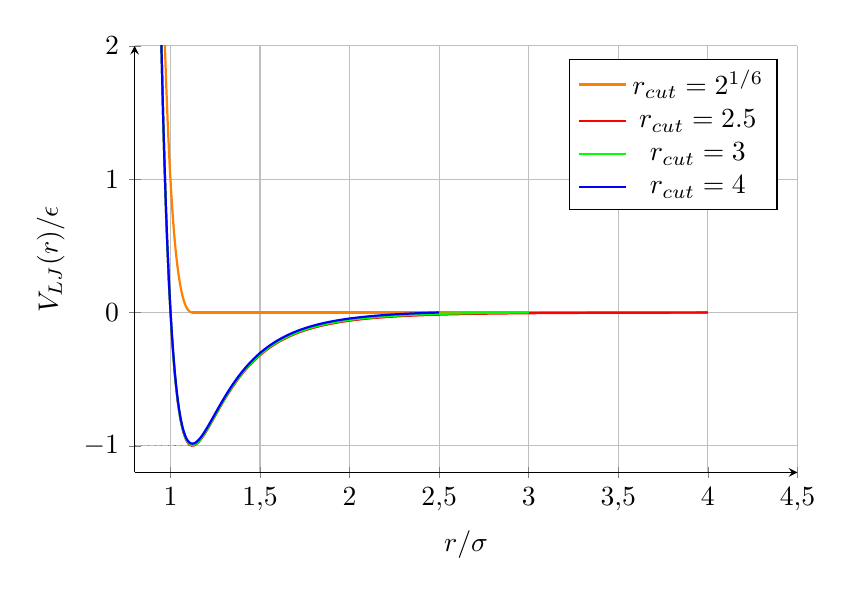
\begin{tikzpicture}
	\begin{axis}[
		% Impostazioni Assi
		axis lines = left,
		xlabel = {$r / \sigma$},
		ylabel = {$V_{LJ}(r) / \epsilon$},
		% Limiti del grafico
		xmin = 0.8, xmax = 4.5,
		ymin = -1.2, ymax = 2.0,
		% Stile
		grid = major,
		width = 10cm,
		height = 7cm,
		legend pos = north east,
		/pgf/number format/.cd,
		use comma,
		1000 sep={}
		]
		
		\addplot [
		domain=1.122:4, 
		samples=200, 
		color=orange, 
		thick,
		]
		{0};
		
		\addplot [
		domain=0.85:4, 
		samples=200, 
		color=red, 
		thick,
		]
		{4*(x^(-12) - x^(-6))};
		\addlegendentry{$r_{cut} = 2^{1/6}$}
		
		\addplot [
		domain=0.85:3, 
		samples=200, 
		color=green, 
		thick,
		]
		{4*(x^(-12) - x^(-6)) + 0.0055};
		\addlegendentry{$r_{cut} =2.5$}
		
		\addplot [
		domain=0.85:2.5, 
		samples=200, 
		color=blue, 
		thick,
		]
		{4*(x^(-12) - x^(-6))+0.016};
		\addlegendentry{$r_{cut} = 3$}
		
		\addplot [
		domain=0.85:1.122, 
		samples=200, 
		color=orange, 
		thick,
		]
		{4*(x^(-12) - x^(-6)) + 1};
		\addlegendentry{$r_{cut} = 4$}
		

		
		% Linea verticale per r_cut = 4

		\draw [gray, dotted] (axis cs:0.8, -1) -- (axis cs:1.122, -1);
		
	\end{axis}
\end{tikzpicture}
\caption{\textit{Lennard-Jones potential cut at different distances $r_{cut}$. Note that cutting the potential at small $r$ will introduce a discontinuity in the $V(r)$, i.e. a delta-shaped instantaneous force which has no physical relevance and can inject spurious energy absorption into the system. To counterbalance this problem, one should just add a constant term $+V_{LJ}(r_{cut})$. This procedure has little effect on $r_{cut} = 4, 3, 2.5$ where $V(r_{cut}) \approx 0$ but must be implemented on $r_{cut} = 2^{1/6}$ where $V_{LJ}(2^{1/6}) = -1$. The resulting potential is also called Weeks-Chandler-Andersen (WSA) potential in the scientific community}}
\label{fig:LJplot}
\end{figure}
\subsection{Energy conservation}
Let $E_0$ be the initial energy of the system:
$$
E_0 = K_0 + V_0 = \sum_i \frac{1}{2}p_i^2(t=0) + \sum_{i\neq j} V_{LJ}(r_{ij}(t=0))
$$
where the $p_i(t=0)$ were sampled from the Maxwell-Boltzmann at temperature $T=1$ thanks to the thermostat phase in LAMMPS and the configuration was chosen at random while keeping sufficient distance between the molecules. The time evolution of the total energy is reported in Fig. \ref{fig:energyLJ} for $\rho = 0.62$ and $\rho = 0.4$. Along with the relative energy variation, Fig. \ref{fig:energyLJ} also displays the behavior of the temperature $T$ as a function of time. 

Overall, the VV integrator has produced valid trajectories and the energy has approximately stayed constant: in the worst scenario (when $r_{cut}=1.12\approx 2^{1/6}$), the relative variation with respect to $E_0$ was about $\approx 0.1\%$, which is a solid result and an usually acceptable value when performing MD simulations. Furthermore, one has to consider that the simulation was run until $10^6$ steps were reached: other more sophisticated integration schemes (e.g. Runge-Kutta methods) would have probably better approximated the system during the initial steps but would have yielded a noticeable and unacceptable energy drift over the course of $1$ million time-steps. 

Let us now analyze individual results. When $r_{cut} = 4$, the energy-conservation plot is surprisingly nice for both $\rho = 0.62$ and $\rho = 0.4$: small energy fluctuations of the order of $10^{-4}E_0$ can still be appreciated, but no overall energy drift is detected. When $\rho = 0.62$ and $r_{cut}=3.0$, we observe an interesting phenomena: the system experiences a small positive drift during the first half of the simulation3 and then stabilizes around a fixed plateau (up to some small fluctuations). This is both a good and a bad news: during the first steps, the integrator has injected a small and unphysical amount of energy into the system, breaking energy conservation. However, this trend eventually came to an end and the integrator regained its ability to maintain the energy stationary. Strictly speaking, to obtain stable and robust results, we should have only considered the system in its stationary phase (even though here the energy is different than the one we started with); however, the drift in energy is well below the acceptable threshold, so we included all the time evolution in the analysis to come. The same reasoning goes for the most unstable configurations with $r_{cut} = 2.5$ and $r_{cut} = 2^{1/6}$, where a stationary phase (meaning no drift, just small fluctuations) is harder to find and multiple drifting phases coexist. Still, the overall energy variation is well bounded within $\approx 0.1\%$, hence we can proceed with our analysis.


Another interesting aspect to study is the time evolution of the temperature $T$ which can (and should) vary over time, since we are in a microcanonical ensemble, not in a canonical one. Overall, we expect a temperature fluctuating around the fixed value $\langle T \rangle=1$, and now the entity of the fluctuations is macroscopic ($\approx 10/20 \%$) and has relevant physical properties. Fig.\ref{fig:energyLJ} partially agrees with this theoretical analysis in all cases, but there are small deviations from the expected behavior of $T(t)$. For example, computing the average $T$ over all MD samples, we always observe a slightly different value with respect to $\langle T \rangle = 1$, suggesting a leak (or an injection) of kinetic energy from (into) the system (Table \ref{table:table2}). This is, however, to be expected: from the analysis of the energy $E(t)$ over time, we observed small inconsistencies due to the imperfect nature of the algorithm. Those spurious and unphysical energy leaks/injections have direct effect on the kinetic energy, and, consequently, on the temperature $T$. As long as we don't measure huge deviations from $\langle T \rangle = 1$, we can safely use those results to build robust analysis.

\begin{table}
	\centering
		\begin{tabular}{|c|c|c|}
		\hline
		$r_{cut}$ &  Average $\bar T$ & St Dev $\sigma_T$\\
		\hline
		$4$ &  1.038 & 0.0320 \\
		$3.5$  &  1.0464 & 0.0320\\
		$2.5$  &  1.0700 & 0.0323\\ 
		$1.122$ & 1.0462 & 0.0282\\
		\hline
	\end{tabular}
		\begin{tabular}{|c|c|c|}
		\hline
		$r_{cut}$ &  Average $\bar T$ & St Dev $\sigma_T$\\
		\hline
		$4$ &  0.9685 & 0.0453\\
		$3.5$  &  0.9775 & 0.0447\\
		$2.5$  &  1.0413 & 0.0394\\ 
		$1.122$ & 1.0493 & 0.0204\\
		\hline
	\end{tabular}
	\caption{\textit{Average temperature and associated standard deviation at different values of $r_{cut}$ when $\rho = 0.62$ (left) and $\rho = 0.4$ (right). }}
	\label{table:table2}
\end{table}

\begin{figure}
	\centering
	\includegraphics[scale = 0.4]{./FIG/energyLJ_0_62.pdf}
	\includegraphics[scale = 0.4]{./FIG/energyLJ_0_40.pdf}
	\caption{\textit{Energy and temperature plots at different cut-off radius $r_{cut}$ when $\rho = 0.62$ (first two rows) and $\rho = 0.4$ (last two rows). The time-step was set to $\Delta t = 0.005$ and the number of steps is $10^6$. Overall, the energy deviations and the average temperature are well behaved and bounded. In the temperatures plots, the average $\bar T$ is represented with a dashed line and the standard deviation with a solid band.}}
	\label{fig:energyLJ}
\end{figure} 


\subsection{Potential and kinetic energy}
Provided our simulations have faithfully conserved the total energy $E(t)$ within reasonable bounds, we can start analyzing other physical properties of interest like the potential and kinetic energy. The resulting histograms for those observables (normalized per number of particles) are reported in Fig.\ref{fig:histoKU}.
\begin{figure}
\centering
\includegraphics[scale = 0.4]{./FIG/hist_kin_pot_LJ_0_62}
\includegraphics[scale = 0.4]{./FIG/hist_kin_pot_LJ_0_4}
\caption{\textit{Histograms for the kinetic energy per particle (on the left) and the potential energy per particle (on the right) at various cut-off distances when $\rho = 0.62$ (top band)} and $\rho = 0.4$ (bottom band)}
\label{fig:histoKU}
\end{figure}
Let us first derive how the kinetic energy histogram should look like. By invoking the equipartition theorem, we can write:
\begin{equation}
	\langle K\rangle = \frac{3}{2}Nk_B \langle T \rangle
\end{equation}
for monoatomic gases. Note this is absolutely independent of the potential shape, even more so from the cut-off radius. Since we work with $k_B = 1$ and $T=1$, we should see a kinetic energy per particle $K = 1.5$ \textit{independent of $r_{cut}$}. The kinetic energy histograms in Fig. \ref{fig:histoKU} are compatible with this computation and closely resemble gaussian distributions, but their average values is slightly different from the expected $K = 1.5$, especially for $\rho = 0.62$ when all the $4$ simulations tend to overestimate the correct value of $K$. I believe this is again a matter of numerical instability of the integrator and a direct consequence of the total temperature drift that was commented in the previous subsection: in fact, one can easily see that the worst results for the kinetic energy (that is, the farthest from $K = 1.5$) were obtained when $\rho = 0.62$ and $r_{cut} = 2.5$, the same set of parameters that yielded the worst temperature average in Table \ref{table:table2}. The average kinetic energies are, however, perfectly correlated with the average measured temperature, so that those two anomalies are intimately linked (recall $\langle k \rangle = \frac{3}{2} \langle T \rangle$).

%Another reason to believe that those mismatches are essentially due to the integrator per se and not on some physically relevant property is that they are more evident when the system is more crowded, i.e. when $\rho = 0.62$. Every time a particle is moved

Now let us analyze the behavior of the potential energy. When $r_{cut} = 4,3,2.5$ the attractive well of the Lennard-Jones potential is kept (Fig.\ref{fig:LJplot}) and allows for the formation of persistent inter-molecules bonds, resulting in negative potential energies per particles. The largest $r_{cut}$ is, the more we keep of the attractive portion of the potential and the final average potential energy per particle gets more and mode negative (until an asymptotic value is reached for $r_{cut} = \infty$). However, if we truncate the potential at $r_{cut} = 2^{1/6}$, we completely remove the attractive property of the Lennard-Jones potential and the molecules simply behave by repelling each other if they get too close one to another. This type of truncation, also called \textit{WCA potential}, is a continuous version of the hard sphere model where particles don't interact with each other apart from the exclusion volume repulsion. The potential energy now becomes positive (but this is simply due to the constant added term we already discussed) and, most importantly, close to $0$, precisely what we would expect from a hard sphere model

Observing Fig.\ref{fig:histoKU}, the average potential energy approaches $0$ but does not vanish completely. This occurs because the WCA potential is steep yet differentiable; consequently, particles with sufficiently high kinetic energy can temporarily penetrate the distance $r<1$, resulting in a significant gain in potential energy. This effect becomes much more evident as the system density increases, since the crowdedness and the reduced free volume forces particles to interact more frequently with their neighbors.

\subsection{Radial distribution function}
Finally, we analyze the radial distribution function $g(r)$ of the system, computed via molecular dynamics simulations using LAMMPS. The results are plotted in Fig.\ref{fig:LJrdf}. 
By setting the cutoff radius to $r_{cut} = 4$, we essentially capture the full range of the interaction; consequently, we observe the typical oscillatory behavior characteristic of the Lennard-Jones potential, where peaks alternate with minima. This structural ordering indicates that the fluid possesses significant short-range order. The first sharp peak corresponds to the nearest-neighbor shell, located approximately at the distance where the Lennard-Jones potential reaches its minimum (around $r \approx 2^{1/6}\sigma$). This implies that particles tend to cluster at this energetically favorable distance.  Subsequent peaks represent further coordination shells (next-nearest neighbors). However, as $r$ increases, these oscillations progressively vanishes and $g(r)$ converges to $1$. This decay implies the absence of long-range order, confirming that the system is indeed in a fluid phase where spatial correlations vanish over long distances but are fundamental at small scales.
\begin{figure}
	\centering
	\includegraphics[scale = 0.4]{./FIG/rdf_LJ_0_62.pdf}
	\includegraphics[scale = 0.4]{./FIG/rdf_LJ_0_40.pdf}
	\caption{\textit{Radial distribution function $g(r)$ for the Lennard-Jones model at different cut-off radius when $\rho =0.62$ (above) and $\rho = 0.4$ (below) }}
	\label{fig:LJrdf}
\end{figure}
On the contrary, when $r_{cut} = 2^{1/6}$ the system essentially behaves as a hard sphere model: hence, the radial correlation completely vanishes when $r>2^{1/6}$ since particles only interact thanks to the excluded volume. Note that the curve for $r_{cut} = 2^{1/6}$ is in agreement with the one in Fig.\ref{fig:g(r)} 

For intermediate cut-off radius, the radial distribution curves are similar to the one obtained for $r_{cut} = 4$, since we are still retaining most of the initial Lennard-Jones potential. This is particularly evident for $\rho = 0.62$ but becomes less noticeable when $\rho = 0.4$, where the three different curves (the one for $r_{cut} = 4, 3, 2.5$) start to become diverge one from another. This is because when $\rho = 0.6$, the typical distance between molecules is $\frac{1}{\rho} \approx 1.6$. It's highly improbable the a pair of particle is found at a distance much larger than $1.6$, hence the effect of a cutoff is negligible (as long as $r_{cut} >> \frac{1}{\rho}$). When $\rho = 0.4$, the typical distance is now $2.5$, hence with our choice of cut-off radius we should start to observe some discrepancies in the three curves. As expected, the larger the value of $r_{cut}$ the higher the first peak gets, since larger $r_{cut}$ implies more attraction between particles (and more short-range structure)
\chapter{Interatomic potentials and thermostats}

\section{Lennard-Jones fluid in the NVT ensemble}
In this chapter, we are going to simulate the dynamics of Lennard-Jones particles with $m = 1$ in a cubic box of fixed length $L$. Distances and energies are rescaled adimensionally in such a way that the parameters $\sigma, \epsilon$ appearing in the Lennard-Jones potential
$$
V_{LJ}(r) = 4\epsilon \Bigl(\Bigl(\frac{\sigma}{r}\Bigr)^{12}- \Bigl(\frac{\sigma}{r}\Bigr)^6\Bigr)
$$
are both set to $1$. 

In the previous sections, I integrated the equations of motion for the $N$-particles system with the help of LAMMPS and focused on the offline analyses of the relevant macroscopic quantities (kinetic and potential energy, radial distribution functions, \dots). Here, I decided to modify the code written for the Monte Carlo simulation of Chapter 1 hence implementing myself a modest Velocity-verlet molecular engine. This was done with the prospect of creating a custom thermostat algorithm over which I could exert more control. In fact, a general MD simulation where the EOMs are integrated numerically through a symplectic algorithm will replicate the behavior of a closed system with no external environment acting upon it. Clearly enough, this implies that the correct statistical ensamble to use when describing such a system is the microcanonical (or NVE) ensemble, since energy is conserved by Hamilton's theorem.

However, in this part of the report we'd like to simulate a many-particles system where we fix the temperature $T$ rather than the energy $E$, thus switching to a canonical description of the problem (NVT ensamble). To achieve that, we need to dip the system into a thermal bath at fixed temperature $T$ that can freely exchange energy with the particles. There exists two classes of algorithms that can reproduce this desired thermal dynamics:
\begin{itemize}
	\item \textit{Non-canonical thermostats}: Non-canonical algorithms correctly fix the system temperature $T$ and are usually easier to implement but fail to faithfully reproduce the canonical ensemble properties that the system should display at thermal equilibrium. In this report, the Berendsen algorithm was implemented. The Berendsen algorithm is a rescaling algorithm: at each time step, we measure the kinetic temperature $T_K$ and rescale the velocities of all particles by a factor $\lambda$:
	$$
	\vec v_{i}' = \lambda \vec v_{i}
	$$
	such that:
	$$
	\lambda^2 = 1 + \frac{\Delta t}{\tau}\frac{T - T(t)}{T(t)}
	$$
	where $T$ is the temperature of the thermal bath (i.e. the target temperature) and $\tau$ is a control parameter that governs the intensity of the thermostat itself: when $\tau = \Delta t$, we will rescale at each time step and the thermostat is strongly coupled to the system. When $\tau >> \Delta t$, the corrections applied to the velocities are negligible and we might not reach the target $T$. Usually, the system takes about $\tau$ time-steps to relax at the desired temperature $T$
	\item \textit{Canonical thermostats:} At variance with the non-canonical ones, canonical thermostats truly represent systems displaying canonical ensemble properties (for example, energy fluctuations distributions). In this report, I've implemented the Andersen thermostat. The fundamental idea behind Andersen thermostat is to couple the system with a thermal bath whose interactions is represented by stochastic collisions with the particles. At each time-step, we randomly select a collection of particles that will experience a collision with the thermal bath: when this happens, their current velocities is completely forgotten\footnote{This is the molecular chaos hypothesis, formulated by Boltzmann long ago. Even though it seemingly defies our deterministic understanding of Newtonian motion, it stands as the backbone of modern statistical mechanics}. The new velocity is sampled from the Maxwell-Boltzmann distribution (which is a Gaussian distribution for the velocity components), enforcing the canonical ensemble. Andersen's thermostat is parametrized by a control parameter $\omega$: at each time-step, the probability that a particle will experience the velocity resetting is $P = \omega \delta T$. The larger $\omega$ is, the stronger the thermostat will couple to the system. 
\end{itemize}

\subsection{Non-canonical vs canonical}

As a first sanity check, let's see if our handmade implementation of the Velocity Verlet with no thermostat really works. It should be enough to test whether the total energy is conserved or not. In Fig. \ref{fig:ThermoNo}, the usual relative energy deviation plot is drawn.  

\begin{figure}
	\centering
	\includegraphics[scale = 0.5]{./FIG//energy_conservation.pdf}
	\caption{\textit{Relative mechanical energy variation for the Velocity-Verlet algorithm implemented (with no thermal bath) versus time. Here, $\Delta t = 0.005$ and $T = 500$.}}
	\label{fig:ThermoNo}
\end{figure}
It's easy to notice a somewhat strange oscillatory trend, the same we observed in Fig.\ref{fig:energyHO}. However, the energy drift with respect to the initial value is on the order of $0.1\%$, a well acceptable value that is also in agreement with LAMMPS simulation (Fig. \ref{fig:energyLJ} but also Fig. \ref{fig:energyHO}).

Next, we can proceed with implementing both Berendsen and Andersen thermostat. 
\subsubsection{Berendsen thermostat}
When using Berendsen thermostat, one can control the intensity of the coupling with the system via the parameter $\tau$ (measured in $\delta t$ units). In Fig.\ref{fig:kinetic_berendsen} we illustrate the temperature $T_K$ histograms varying $\tau$ fixing the target temperature $T = 1$ (in adimensional units).\footnote{Clearly enough, the instantaneous temperature can be obtained by measuring the kinetic energy}

When $\tau = 1$, meaning $\tau = \Delta t$, we fallback to a standard velocity-rescaling algorithm. The coupling with the system is extremely aggressive and forces the temperature to be exactly $T = 1$ at each time-step, making the histogram become a Delta dirac distribution around the expected desired value with no fluctuations. When $\tau$ gets larger, the thermal bath interaction gets gentler and temperature is now free to fluctuate around $T = 1$\footnote{We only consider $t > \tau$ to build histograms, since the Berendsen procedure takes time to make the system reach equilibrium. Having $10000$ total timesteps at disposal, it seemed reasonable to stop at $\tau = 2000$. }. However, the coupling becomes so weak that the system takes a large time to thermalize and, when $\tau = 100000$, the resulting histogram is not even centered around $T = 1$, meaning that the system had not yet reached equilibrium. 


\begin{figure}
	\centering
	\includegraphics[scale = 0.55]{./FIG//berendsen_kinetic.pdf}
	\caption{\textit{On the left, histogram of sampled temperature $T_K$ for various value of $\tau$ (Berendsen thermostat). On the right, standard deviation of those histograms as a function of $\tau$. The dotted line represent the analytical value of $\sigma_T$ that one would expect in a canonical ensemble and the empirical value extracted from previous chapters in the microcanonical ensemble. The simulation was run with $N = 200, \Delta t = 0.005, T = 500$.}}.
	\label{fig:kinetic_berendsen}
\end{figure}

In Fig. \ref{fig:kinetic_berendsen} it is also reported the behavior of the standard deviation $\sigma_T$ as a function of $\tau$. In the canonical ensemble, we'd expect:
$$
\sigma_T^2 = T^2 \frac{2}{3N}
$$
Instead, what we observe in Fig.\ref{fig:kinetic_berendsen} is a completely different scenario. The standard deviation is not independent of $\tau$ (which has no physical relevance in this problem, being a simple algorithmic parameter) and steadily grows as $\tau$ gets larger until a plateau $\sigma_T \approx 0.04$ is reached, far enough from the expected $\sigma_T^2 = T^2 \frac{2}{3N} \approx 0.06$ when $N = 200$. Interestingly enough, when $\tau$ is large the standard deviation gets closer to the values reported in Tab.\ref{table:table2} for $r_{cut} = 2.5$ and $\rho = 0.4$ that were obtained in the NVE ensemble. This is to be expected: when $\tau$ is exceedingly large, the Berendsen coupling is so weak that no thermalization really occurs. The rescaling effect is so small that particles virtually conserve their velocities and, consequently, their energy, behaving as if they were in a microcanonical ensemble.

\subsubsection{Andersen thermostat}
Andersen thermostat is not based on a rescaling procedure, but rather on a stochastic modeling of particles collisions with a fixed temperature thermal bath. The process is governed by the parameter $\omega$: larger $\omega$ implies higher collision probability, hence stronger coupling with the system. In Fig. \ref{fig:kinetic_andersen} we show the same plots reported in Fig. \ref{fig:kinetic_berendsen} when using an Andersen thermostat upon varying $\omega$. 
\begin{figure}
	\centering
	\includegraphics[scale = 0.55]{./FIG//andersen_kinetic.pdf}
	\caption{\textit{On the left, histogram of sampled temperature $T_K$ for various value of $\omega$ (Andersen thermostat). On the right, standard deviation of those histograms as a function of $\omega$. Again, the dotted line represent the analytical value of $\sigma_T$ that one would expect in a canonical ensemble and the empirical value extracted from previous chapters in the microcanonical ensemble. The simulation was run with $N = 200, \Delta t = 0.005, T = 500$.}}
	\label{fig:kinetic_andersen}
\end{figure}
When $\omega$ is small, the coupling is so weak that the simulation is virtually equivalent to a energy-conserving integration, i.e. a microcanonical ensemble (and the standard deviation of the resulting distribution stabilizes around the microcanonical one obtained in Tab.\ref{table:table2}). What do we mean by "small" $\omega$? At each time-step, particles have a probability $P = \omega \Delta t$ of experiencing a collision and having their velocity resampled. Given $N$ particles, the expected number of collisions per unit time is $\mathcal{N} = \omega N \Delta t$. The thermostat start influencing the system when $\mathcal{N} \approx O(1)$, so that:
$$
\omega \approx \frac{1}{N \Delta t}
$$
For the displayed simulations, $N = 200$ and $\Delta t = 0.005$, hence $\omega$ must be approximately $1$ to have a reasonable thermostat (and indeed this is what we observe in Fig.\ref{fig:kinetic_andersen}: when $\omega = 10^{-4}, 10^{-3}, 10^{-2}$ the histograms are not even centered around $T = 1$ and the variance is closer to the one associated to the microcanonical ensemble). When $\omega > 0.1$, the thermostat starts kicking in and allows the system to thermalize at the target temperature $T = 1$. Even more, the $T_K$ distributions seem to be independent enough from $\omega$ and the standard deviation $\sigma_T$ fluctuates around the expected value $\sigma_T^2 = T^2 \frac{2}{3N}$.

Now that we have what seems to be a canonical thermostat, let's see how changing the particles number $N$ affects the width of the temperature histogram. We'll set $T = 2$ and select $\omega$ from the range of acceptable values highlighted in Fig. \ref{fig:kinetic_andersen}. Results are shown in Fig. \ref{fig:andersenN} and display both the histograms (at fixed $\omega = 1$) and a logarithmic-logarithmic plot of $\sigma_T$ versus $N$ when $\omega = 1$ and $\omega = 10$ (averaging over $10$ realizations). The plot is convincing and solid evidence for the scaling relation $\sigma_T^2 = T^2 \frac{2}{3N}$, providing confirmation of the canonical nature of the Andersen thermostat.

\begin{figure}
	\centering
	\includegraphics[scale = 0.55]{./FIG//andersen_size.pdf}
	\caption{\textit{On the left, histogram of sampled temperature $T_K$ for various value of $N$ number of particles (Berendsen thermostat, coupling $\omega = 1$.). On the right, standard deviation of those histograms as a function of $N$ using two distinct values of $\omega$. The scaling behavior $\sigma_T \sim O(T^{-2})$ is shown with a dotted line. Both simulations were run with $N = 200, \Delta t = 0.005, T = 500$.}}
	\label{fig:andersenN}
\end{figure}
The same plot concerning Berendsen algorithm is reproduced in Fig. \ref{fig:berendsenN} when $\tau = 10$ or $\tau = 100$. The situation here is quite different and the desired  scaling behavior for $\sigma_T$ is definitely not obeyed by Berendsen thermostat, providing hint of its non-canonical properties.
\begin{figure}
	\centering
	\includegraphics[scale = 0.55]{./FIG//berendsen_size.pdf}
	\caption{\textit{On the left, histogram of sampled temperature $T_K$ for various value of $N$ number of particles (Andersen thermostat, coupling $\tau = 10$.). On the right, standard deviation of those histograms as a function of $N$ using two distinct values of $\tau$. The scaling behavior $\sigma_T \sim O(T^{-2})$ is shown with a dotted line. Both simulations were run with $N = 200, \Delta t = 0.005, T = 500$.}}
	\label{fig:berendsenN}
\end{figure}


\section{The Flying Ice Cube effect}
The \textit{Flying ice cube effect} is a numerical artifact common in velocity rescaling based thermostats that can cause violation in the equipartition theorem.

In this section, we will consider a FCC crystal (as provided in the Moodle). Atoms ($m = 1$) interact through a standard normalized Lennard-Jones potential where  $r_{cut} = 3.5, \sigma = 1, \epsilon = 1$. The temperature is set to $k_B T = 1$. 

\paragraph{Crystalline structure} Before considering the flying ice cube effect, let us explore the static structure of the atoms displaying the radial distribution function $g(r)$ (Fig.\ref{fig:rdf})

\begin{figure}
	\centering
	\includegraphics[scale =0.66]{./FIG//RDF_plot_crystalline.pdf}
	\caption{\textit{Radial distribution function for the initial configuration (FCC32 and FCC108) provided in the Moodle}}
	\label{fig:rdf}
\end{figure}

The two functions refer to the same FCC structure at the same numerical density with different particles number ($N = 108, N = 32$). The curves are pretty much perfectly aligned and they both display the standard peaks and valleys typical in a crystalline structure, in particular a FCC lattice. The sudden peak when $N = 32, r \approx 3.1$ is just an artifact and is due to the fact that the simulation was run in a box of size $L \approx 3.1$. It makes no sense to consider a $g(r)$ when $r > L$, the simulation length (and the peak at $r = L$ is due to the fact that the particle has found itself).

\paragraph{Equipartition theorem}
The equipartition theorem states that, at thermal equilibrium, each quadratic degrees of freedom appearing in the Hamiltonian of the system has an average energy associated of $\frac{1}{2}k_B T = \frac{1}{2}$ (with $T=1$). 

For example, only considering the kinetic energy $K$:
$$
K = \frac{1}{2}\sum_i^N |\vec v_i|^2 =  \frac{1}{2}\sum_i^N (v_x^{(i)})^2 + (v_y^{(i)})^2 +(v_z^{(i)})^2
$$
This is a sum on $3N$ purely quadratic terms and, invoking equipartition theorem, we expect that each particle will have on average a kinetic energy of $3\times 0.5 = 1.5$ (a fact that we have already demonstrated). 

To better see the flying ice cube effect, let's rewrite the kinetic energy as:
$$
K = \frac{1}{2}\sum_i^{N-1} |\vec v_i|^2 + \frac{1}{2}|\vec v_{CM}|^2
$$
where $\vec v_{CM}$ is the velocity of the center of mass. What we've done is a simple permutation of degrees of freedom: instead of considering all of $3N$ particles velocity components, we' deal with $3N-3$ degrees of freedom coming from $N-1$ particles and an additional $3$ degrees of freedom accounted by the center of mass displacement. Those perspective are perfectly equivalent.

Interpreting $\vec v_{CM}$ as a degree of freedom, that its associated (kinetic) energy should be on the order of $3\times 0.5$ too. Moreover, if we consider the ratio:
$$
\frac{K_{CM}}{K_{tot}}
$$ 
that is the ratio between the kinetic energy coming from the center of mass and the total kinetic energy, then we'd expect by equipartition theorem:
$$
\frac{K_{CM}}{K_{tot}} \approx\frac{3}{3N-3} = \frac{1}{N-1}
$$ 

Let us now verify whether the numerical thermostats obey this relation. Results are shown in Fig.\ref{fig:equipartition}

It's quite easy to see that Andersen's thermostat closely reproduces the expected kinetic ratio on the order of $1/N-1 \approx 0.01$ in at least two orders of magnitude for its control parameter $\omega$. However, when using a velocity-rescaling algorithm, the situation is quite different. For any value of $\tau$ used in the simulations, the thermostat eventually transferred all the kinetic disordered energy into well-ordered macroscopic kinetic energy (i.e. center-of-mass motion). The overall kinetic energy $K_{tot}$ is still correct, but the system is not distributing in an equal way its energy into the internal available degrees of freedom (the system literally starts to \textit{fly away}, gaining a macroscopic ordered velocity that has no physical relevance)

\begin{figure}
	\centering
	\includegraphics[scale =0.5]{./FIG//equipartition.pdf}
	\caption{\textit{Ratio between kinetic energy of the center of mass and total kinetic energy when using Berendsen thermostat (below) or Andersen thermostat (above)}}
	\label{fig:equipartition}
\end{figure}

\chapter*{Multiple Markov chains and the Multiple Histogram Method}

\section{Multiple Markov chain}

We will consider of $N = 64$ identical particles in a $2$-dimensional square box of side $L$ with periodic boundary condition. We will not use $L = 6$ as suggested, since this will create an impossible configuration (there's no room to accomodate all $N$ particles); instead, we chose $L =16$, so that $\rho = 0.25$. 
The pair interaction potential is the usual square-well volume excluding potential:
\begin{equation}
	U(r) = 
	\begin{cases}
		+\infty \mbox{ for } r < R_c \\
		-\epsilon \mbox{ for } R_c < r < R_a \\
		0 \mbox{ for } r > R_a
	\end{cases}
\end{equation}
where $R_c = 1, \varepsilon = 1, R_a = 1.5$ and $k_B = 1$.

In this first task, we will implement a Metropolis Monte Carlo algorithm for this system to simulate in parallel replicas of the system
at different inverse temperatures:
$$
\beta \in \{1, 1.2, 1.4, 1.6,  1.8, 2, 2.2, 2.4\}\footnote{The temperatures used here are different from the one proposed in the homework assignment. This is because the system where $L =16$ undergoes a phase transition when $T \approx 0.6$ or $\beta \approx 1.6$}.
$$

Within each chain, the particles move through single-particle displacements. Moves that produce overlaps $r < R_c$ are automatically rejected, otherwise they are accepted with the Metropolis rule. Every $n_{swap}$ sweeps
(where a sweep corresponds to $N$ attempted single moves in each of the $K = 8$ Markov chains), attempt a swap of configurations between randomly picked neighboring replicas $k$ and $k + 1$, with acceptance probability as to fulfill detailed balance for the joint probability density functions of all $8$ systems.

\paragraph{Code implementation}
The vast majority of the code for this assignment was simply copied from the codebase of Exercise 1: The Hard Sphere model (where the interaction range was set to $R_a = 1.5$). Instead of launching just one Markov chain, we spawn a set of $K = 8$ threads that will each run an independent instance of a Markov chain with a specific temperature $\beta$. Each thread will run in parallel with the others until $n_{swap}$ steps have been performed. When this happens, all thread synchronize and the master thread will handle the Metropolis swap between two randomly selected configurations. 

Let us first verify as a sanity check that adding the parallel tempering procedure provides stable and reasonable results. In Fig.\ref{fig:HistogramsParallelTempering} we illustrate the potential energy histograms and trace plots for $3$ distinct values of $\beta$ ($1.2, 1.6, 2.2$, meaning $T \approx 0.83, 0.625, 0.45$), with and without parallel tempering. The total number of MC steps is set to $N_{MC} = 10^6$ and $n_{sweep} = 1000$, so that, on average, each configuration will stay at a fixed temperature for about $8000$ MC steps and should experience $\approx 100$ swaps during a full run.

\begin{figure}
	\centering
	\includegraphics[scale = 0.55]{./FIG/Energy_Histograms.pdf}
	\caption{\textit{efwf}}
	\label{fig:HistogramsParallelTempering}
\end{figure}

Having a closer look at Fig.\ref{fig:HistogramsParallelTempering}, one can easily see that the histograms and trace plots obtained using parallel tempering are quite identical (up to normal stochastic fluctuations) to the one generated by single independent Markov chains (obtained by setting $n_{sweep} = N_{MC}$), confirming that the implementation of the algorithm was successful. Furthermore, both algorithms converge nicely to the target distribution (in this case, the joint PDF for all Markov chains) as indicated by the initial transient in the $\beta = 2.2$ panel, hence we are effectively producing equilibrated samples at a fixed temperature. The reasons why we don't see any difference is because the temperatures here are still sufficiently high and there is no significative benefit in using parallel tempering against standard Metropolis (we will explore the low temperatures regime in the next paragraph). 

\paragraph{Energy and specific heat}
Now that we have multiple samples extracted from the equilibrium Boltzmann distribution at different $\beta_k$, we can compute various observables of interest such as the potential energy per particle $U/N$ and the specific heat per particle $C/N$\footnote{As highlighted in the first chapter, a MC simulation can only "sample" the configurational phase space of the system, since we are totally neglecting the momenta phase space dynamics. When we talk about energy, we are actually referring to the \textit{potential energy}. The specific heat is thus computed as a measure of fluctuations over the \textit{potential energy} distribution and not on the full energy distribution. However, this is not a problem as far as we're concerned: if we are looking for a divergence in the specific heat and we don't care about the correct numerical values, then considering only $U$ should be enough, because the critical singularity is due to the fact that the system suddenly changes geometry (from disordered gas to ordered fluid) and this can be seen by inspecting the potential energy.}. Results are shown in Fig. \ref{fig:EnergySpecificHeatPT}

\begin{figure}
	\centering
	\includegraphics[scale = 0.5]{./FIG/Energy_SpecificHeat_PT.pdf}
	\caption{\textit{ed}}
	\label{fig:EnergySpecificHeatPT}	
\end{figure}

The average potential energy of the system decreases monotonically as the temperature gets lower, as expected. The specific heat plot reveals a phase transition around $T \approx 0.55$. This corresponds to a liquid-gas phase transition: when the temperature is high enough (above the critical value, which is defined only in the thermodynamic limit), the particles have sufficient thermal energy to travel freely in the square box in a disordered gas phase. The residual energy we observe (for $T \to \infty$) is simply due to the finiteness of the box, forcing particles to interact temporarily (Van der Waals interactions). On the contrary, when $T < T_c$ the energy drops down and it's more thermodynamically favorable for the system to condense and form denser cluster of liquid where particles are permanently surrounded by other particles.

We can use OVITO as we did in the previous sections to visually inspect some configurations at different temperature and verify whether a phase transition is really occurring (Fig.\ref{fig:OVITOPT}). As expected, when $\beta$ is high (low $T$) the system evolves towards liquid configurations, where particles cluster together in droplets. As $\beta$ decreases, those droplets become more and more "fuzzy" (coexistence region, stable liquid droplets coexist with a stable disordered gas) until a totally gaseous phase is reached.

\begin{figure}
	\centering
	\includegraphics[scale = 0.1]{./FIG/beta2.2_Swap}
	\includegraphics[scale = 0.1]{./FIG/beta2.4_Swap}
	\includegraphics[scale = 0.1]{./FIG/beta2.0_Swap}
	\includegraphics[scale = 0.1]{./FIG/beta1.8_Swap}
	\includegraphics[scale = 0.1]{./FIG/beta1.6_Swap}
	\includegraphics[scale = 0.1]{./FIG/beta1.4_Swap}
	\includegraphics[scale = 0.1]{./FIG/beta1.2_Swap}
	\includegraphics[scale = 0.1]{./FIG/beta1.0_Swap}
	\caption{\textit{edec}}
	\label{fig:OVITOPT}
\end{figure}

\paragraph{Swap rates and Parallel tempering}
In this paragraph, we will delve deeper into the parallel tempering procedure. In previous simulations, we always used $N_{MC} = 10^6$ and $n_{swaps} = 1000$, ensuring a fair number of possible swaps between configurations. In particular, during one of the run, we measured:
\\
$$
\mbox{ Total swap acceptance ratio: } 31.9 \%
$$
\begin{itemize}
	\centering
	\item Chain 0 ($\beta=1$): 53 swaps.
	\item Chain 1 ($\beta=1.2$): 92 swaps.
	\item Chain 2 ($\beta=1.4$): 73 swaps.
	\item Chain 3 ($\beta=1.6$): 61 swaps.
	\item Chain 4 ($\beta=1.8$): 72 swaps.
	\item Chain 5 ($\beta=2$): 97 swaps.
	\item Chain 6 ($\beta=2.2$): 121 swaps.
	\item Chain 7 ($\beta=2.4$): 69 swaps.
\end{itemize}
The swap rate is satisfactory. Each chain experienced an average of $\approx 80$ swaps whose length was about $10^6 / 80 \approx 12000$ Monte Carlo steps each. At a first glance, there seems to be a significative imbalance between the number of swaps at each value of $\beta$. However, this can be easily explained by considering that, in our implementation of the parallel tempering algorithm, we only swap between neighboring temperatures, penalizing extreme values ($\beta = 1, \beta = 2.4$) that only experience about half of the expected number of swaps. But there's more: when $\beta = 1.6$, the number of exchanges is at its lowest (ignoring border values). This might seem strange at first, considering that the Metropolis acceptance probability depends on $\Delta \beta$ which is fixed here. However, one should not forget that it also depends n $\Delta E$, i.e. the energy difference between configurations. Around the critical point, it might happen that the two candidate configurations are in two different phases, one liquid the other one gaseous, hence $\Delta E$ is larger compared to chains where $\beta$ is far from the critical point (and both configurations are in the same phase). 

In Fig.\ref{fig:PathPT}, we can appreciate the swaps taking place from the perspective of a fixed Markov chain (defined according to the initial temperature). The parallel tempering algorithm allows the diffusion of each configuration over time from cold to hot conditions and back.

\begin{figure}
	\centering
	\includegraphics[scale = 0.55]{./FIG/TemperaturePaths.pdf}
	\caption{\textit{ioin}}
	\label{fig:PathPT}
\end{figure}




\paragraph{Low temperatures regime}
Up until now, there was no reason to believe parallel tempering can actually be superior with respect to the usual Metropolis algorithm when it comes to sample from Boltzmann equilibrium distributions. In Fig. \ref{fig:HistogramsParallelTempering}, both procedures (with and without parallel tempering) seem to reproduce the same curve, up to statistical errors. Let's see what happens when the chosen temperatures $\beta_k$ are lower than before:
$$
\beta \in \{4,5,6,7,8,9,10,11\}
$$
Results concerning energy histograms and trace plots are shown in Fig.\ref{fig:HistogramsLowt}. When $\beta = 4 (T = 0.25)$, there still is no sensible difference when using parallel tempering. However, a completely different scenario emerges when $\beta = 8$ or $\beta = 11$ (corresponding to $T = 0.125$, $T = 0.09$). Both simulations seem to have found a stationary state, i.e. a minimum of the free energy, even though the average (potential) energy per particle is definitely not the same. What's the reason behind this strange behavior? Why is the average energy per particle lower when parallel tempering is used?

The reason is that, when $T$ is extremely low, the free energy landscape becomes particularly complex. Imagine a configuration where particles are distributed in two distinct but similar clusters (or droplets). This is not yet the equilibrium configuration, but rather a \textit{metastable state}. To further decrease the energy (which is essential in the low $T$ regime, where the entropic term is negligible), the system should make the two droplets merge. For this to happen, particles on the boundary of one cluster should evaporate and then attach to the other droplet. The difference in energy associated to the evaporation of an external particle is about $\Delta E = -3$ ($3$ particles on one side, none on the other). When $\beta = 8$, for example, the associated Metropolis acceptance rate for this move is $\exp(-3 \cdot 8) = \exp(-24) \approx 10^{-11}$. Hence, if the system collapses into one of these multi-cluster metastable states, the usual Metropolis algorithm is unable to nudge away from these configurations. This is also called \textit{quasi-ergodicity}, i.e. the fact that a small portion of the phase space is explored but never abandoned to reach other relevant portions because the intermediate states are very unlikely. 

\begin{figure}
	\centering
	\includegraphics[scale = 0.55]{./FIG/Energy_Histograms_LowT}
	\caption{\textit{ded}}
	\label{fig:HistogramsLowt}
\end{figure}

With parallel tempering, this problem is solved by frequently switching configurations (provided this swapping rule obeys detailed balance). The system should now be able to relax to low energy states, as it should be in the low temperature regime. In Fig.\ref{fig:comparaison}, this difference is illustrated with two snapshots coming from the same $\beta$ with and without parallel tempering.

\begin{figure}
	\centering
	\includegraphics[scale = 0.255]{./FIG/PT}
	\includegraphics[scale = 0.2]{./FIG/NoPT}
	\caption{\textit{ec}}
	\label{fig:comparaison}
\end{figure}

\paragraph{A new phase transition}
Let's plot the average (potential) energy per particle and the specific heat per particle at low temperatures. Results are shown in Fig.\ref{fig:energy_lowT}
\begin{figure}
	\centering
	\includegraphics[scale = 0.5]{./FIG/Energy_SpecificHeat_LowT.pdf}
	\caption{\textit{ced}}
	\label{fig:energy_lowT}
\end{figure}
The supremacy of parallel tempering is now much more evident. The green line (no parallel tempering) is completely wrong when $T < 0.22$; the correct behavior is recovered only by the blue line. An interesting feature that can be observed by inspecting Fig.\ref{fig:comparaison} is that the specific heat displays a new peak around $T \approx 0.2$.

This should be caused by a brand new phase transition, from a cluster liquid phase to a \textit{cluster crystalline structure}. Particles are still trapped in dense clusters, but now they arrange in a rigid crystalline structure which is denser and that further decreases the potential energy of the system (Fig.\ref{fig:secondPhaseTransition})

\begin{figure}
	\centering
	\includegraphics[scale = 0.14]{./FIG/beta3.0}
	\includegraphics[scale = 0.14]{./FIG/beta4.0}
	\includegraphics[scale = 0.14]{./FIG/beta5.0}
	\includegraphics[scale = 0.14]{./FIG/beta6.0}
	\vspace{5pt}
	\includegraphics[scale = 0.14]{./FIG/beta7.0}
	\includegraphics[scale = 0.14]{./FIG/beta8.0}
	\includegraphics[scale = 0.14]{./FIG/beta9.0}
	\includegraphics[scale = 0.14]{./FIG/beta10.0}
	\caption{\textit{edec}}
	\label{fig:secondPhaseTransition}
\end{figure}

We can clearly see that particles now form densely-packed clusters where every atom has $8$ neighbors (i.e. a \textit{crystal}). When $T \to 0$, this would mean that we should observe a potential energy of $U/N = -4$, which is not the case as depicted in Fig.\ref{fig:energy_lowT}. This is simply due to a finite size effect: particles located at the borders cannot create bonds with $8$ neighbors, hence increasing by a small amount the total energy of the system\footnote{When $N\to\infty$, the number of border particles become negligible when compared to the number of bulk particles, so we should be able to asymptotically reach $U(T = 0) = -4$ performing a thermodynamic limit.}


\section{Multiple Histogram Method (MHM)}

\chapter*{Gillespie algorithm}
\section{The Brusselator model}
In this chapter we will implement the Gillespie algorithm to simulate the Brusselator model. The transition rates for a state $C =(X, Y)$ are given by:
\begin{equation}
	\begin{cases}
		w_1 = a \Omega \mbox{ for } (X,Y)\to(X+1, Y) \\
		w_2 = X \mbox{ for } (X,Y)\to(X-1, Y) \\
		w_3 = \frac{1}{\Omega^2}X(X-1)Y \mbox{ for } (X,Y)\to(X+1, Y-1) \\
		w_4 = bX \mbox{ for } (X,Y)\to(X-1, Y+1)
	\end{cases}
	\label{eq:Brusselator}
\end{equation}
Run some simulations using $a = 2, b = 5$ and for different volume sizes:$\Omega = 10^2, 10^3, 10?4$.

\subsection{Mean field analysis}
Before delving into the implementation and analysis of the Gillespie algorithm for the Brussellator, let us perform a mean-field analysis of the problem. This is equivalent to a simulation where no statistical fluctuations are allowed and the evolution of the intensive state variables $(x,y) = (\frac{X}{\Omega}, \frac{Y}{\Omega})$ is governed by a set of ODEs:
\begin{equation}
	\begin{cases}
		\dot{x} = a - (b+1)x + x^2 y \\
		\dot{y} = bx - x^2 y 
	\end{cases}
\end{equation}
The fixed point of the system is defined by:
\begin{equation}
	\begin{cases}
		0 = a - (b+1)x + x^2 y \\
		0 = bx - x^2 y 
	\end{cases}
\end{equation}
which implies $(x^*, y^*) = (a, \frac{b}{a})$. To evaluate the behavior of the system close to the fixed point, we will compute the jacobian:
\begin{equation}
	J(x^*, y^*) = 
	\begin{pmatrix}
		b-1 & a^2 \\
		-b & -a^2
	\end{pmatrix}
\end{equation}
its eigenvalues are:
\begin{equation}
	\lambda_{1,2} = \frac{b-1-a^2 \pm \sqrt{(b-1-a^2)^2-4a^2}}{2}
\end{equation}
The eigenvalues are real or complex according to the sign of $(b-1-a^2)^2 - 4a^2$. In fact,
\begin{itemize}
	\item Case 1 ($b -1 -a^2 < 2a$): the argument of the square root is negative, hence the eigenvalues are complex. The stability of the system depends on the real part: if $ b - 1-a^2 > 0$, then the fixed point is unstable. If $ b - 1-a^2 < 0$, the stationary state is stable and trajectories spirals around it until convergence.
	\item Case 2 ($b -1 -a^2 > 2a$): the argument of the square root is positive. The eigenvalues are thus real. Rewriting the numerator as $(b-1-a^2) (1\pm\sqrt{1-\frac{4a^2}{(b-1-a^2)^2}})$ and since $b -1 -a^2 > 2a > 0$, both eigenvalues are positive, causing instability.
\end{itemize}
In conclusion, the stability of $(x^*, y^*)$ depends on $b < 1+a^2$. In this specific case, given $a = 2$ and $b = 5$ the system should converge to a \textit{limit cycle}. The real part of the eigenvalues is precisely zero, hindering an exponential decay away from or towards the fixed point. 

\subsection{Gillespie algorithm}
Now let's introduce the stochasticity implementing the Gillespie algorithm for the continuous time Markov chain defined by Eqs. \ref{eq:Brusselator}. A minimal version of the implemented code is proposed here:
\begin{lstlisting}[language=python]
	def brusselator_gillespie(Omega, a = 2.0, b = 5.0, t_max = 50.0):
		# Initial value
		X, Y, t = int(a * Omega), int(b * Omega), 0
		T, X_hist, Y_hist = [0.0], [X], [Y]
		
		while t < t_max:
			w1 = a * Omega
			w2 = X
			w3 = (1.0 / Omega**2) * X * (X - 1) * Y
			w4 = b * X
			W_tot = w1 + w2 + w3 + w4
			
			if W_tot == 0: break
			# Extract the residence time
			t += -np.log(np.random.random()) / W_tot
			# Extract where to jump to
			r = np.random.random() * W_tot
			
			if r < w1:
				X += 1
			elif r < w1 + w2:
				X -= 1
			elif r < w1 + w2 + w3:
				X += 1; Y -= 1
			else:
				X -= 1; Y += 1
			
			T.append(t); X_hist.append(X); Y_hist.append(Y)
		
		return np.array(T), np.array(X_hist)/Omega, np.array(Y_hist)/Omega
\end{lstlisting}
In Fig.\ref{fig:BrusselatorTimeSeries} the time evolution of the state variable $x(t) = X(t)/\Omega, y(t) = Y(t)/\Omega$ are represented for three different choices of $\Omega \in [100, 1000, 10000]$. In Fig.\ref{fig:BrusselatorPortrair} the same plots are represented in the phase plane.

For small values of $\Omega$, the system is dominated by statistical fluctuations. While the dynamics follows the general path of the limit cycle around the fixed point $(a, \frac{b}{a}) =(2, 2.5),$ it undergoes significant stochastic deviations. Consequently, the resulting limit cycle appears aperiodic, disordered and diffuse. As $\Omega$ increases, the time series becomes progressively more regular (once the initial transient phase has decayed) and settles onto a smooth, periodic limit cycle. The black line highlights the solution to the associated ODEs, representing the mean-field approximation. As expected, the stochastic simulation converges to this deterministic solution when $\Omega$ becomes large (i.e., approaching the thermodynamic limit where $X, \Omega \to \infty$ and $X / \Omega$ remains finite)


\begin{figure}
	\centering
	\includegraphics[scale = 0.4]{./FIG/Brusselator_TimeSeries.pdf}
	\caption{\textit{Time evolution for the state variable $x(t), y(t)$ when $\Omega = 10^2, 10^3, 10^4$. The black dotted lines indicate the mean-field solution for the Brusselator, obtained integrating the corresponding ODEs. When $\Omega$ is small, the oscillations are wild and irregular, but they follow the typical behavior of a limit cycle. As $\Omega$ increases, the trajectories collapse onto the mean-field solution as expected.}}
	\label{fig:BrusselatorTimeSeries}
\end{figure}

\begin{figure}
	\hspace{-2cm}
	\includegraphics[scale = 0.415]{./FIG/Brusselator_PhaseSpace.pdf}
	\caption{\textit{Same as in Fig. \ref{fig:BrusselatorTimeSeries} but viewed in the phase plane. The red dot is the fixed point, which is at the boundaries between stability and instability when $b = 5, a =2$ (Hopf bifuraction). Trajectories gravitate around the fixed point: smaller $\Omega$ implies irregular and rough orbits while larger $\Omega$ converge to the regular mean-field limit cycle (leftmost plot). }}
	\label{fig:BrusselatorPortrair}
\end{figure}

%\setcounter{chapter}{5}




\end{document}
